\documentclass[t,% Place text of slides at the (vertical) top of the slides
brazilian,% Brazilian Portuguese, FTW!
11pt,% Standard font size
aspectratio=169,% Aspect ratio 16:9 (widescreen)
table% xcolor option
]{beamer}

\setbeamercolor{footnote mark}{fg=red}

\usetheme{Boadilla}
\setbeamertemplate{navigation symbols}{}
\setbeamertemplate{frametitle continuation}{}
\setbeamertemplate{page number in head/foot}[framenumber]
\setbeamertemplate{enumerate items}[default]
\setbeamertemplate{itemize items}[circle]
\setbeamercovered{transparent}
\setbeamerfont{frametitle}{size=\normalsize}

\usepackage{babel}
\usepackage[utf8]{inputenc}
\usepackage[T1]{fontenc}
\usepackage{lmodern}

\usepackage{graphicx}
\setkeys{Gin}{keepaspectratio}

\usepackage{amssymb,amsfonts,amsmath}
\usepackage{mathtools}

\usepackage{siunitx}
\sisetup{locale = FR}

\usepackage{tikz}
\usetikzlibrary{calc}

\usepackage{pgffor}
\usepackage{etoolbox}

% \usepackage{pgfcalendar}
% \usepackage{xstring}
% \usepackage{xcolor}
% \usepackage{colortbl}

\usepackage{tcolorbox}

\usepackage[calc]{adjustbox}

\usepackage{pgfplots}
\pgfplotsset{compat=1.18}

\newcommand{\esima}{\textordfeminine }
\newcommand{\esimo}{\textordmasculine }

\newcommand{\vboxcorr}[2]{%
    \resizebox{!}{\totalheight-#1}{#2}%
}
\newcommand{\hboxcorr}[2]{%
    \resizebox{\width-#1}{!}{#2}%
}

% \usetikzlibrary{decorations.pathmorphing}
\usetikzlibrary{patterns}

\DeclareMathOperator{\sen}{sen}

\def\Disciplina{Física Geral II}
\def\Professor{Rodrigo de Farias Gomes}
\def\Periodo{Período 2025.1}

\title{\Disciplina}
\author{\Professor}
\date{\Periodo}

\begin{document}

\begin{frame}
    \titlepage
\end{frame}


\begin{frame}{Apresentação}
    \begin{itemize}
        \item Professor {\fontfamily{augie}\selectfont Rodrigo de Farias Gomes}
        \item Telefone (somente mensagens): (92) 9 9405-1724
        \item E-mail: shpnft@gmail.com
        \item Sala: 201b, Bloco E (2\esimo{} pavimento)
    \end{itemize}
\end{frame}

\begin{frame}{Ementa de \Disciplina}
    \begin{itemize}
        \item Equilíbrio estático
        \item Oscilações
        \item Fluídos
        \item Ondas em meio material
        \item Ondas sonoras
        \item Temperatura e calor
        \item 1\esima{} Lei da termodinâmica
        \item Teoria cinética dos gases
        \item 2\esima{} Lei da termodinâmica
        \item Ciclo de Carnot
    \end{itemize}
\end{frame}

\begin{frame}[c]{Livro texto}
    \centering
    \begin{tikzpicture}
        \node (Halliday) at (0,0) {
            \includegraphics<1>[height=\textheight-29pt]{images/halliday_9.png}
            \includegraphics<2->[height=\textheight-29pt]{images/halliday_10.png}
        };
        \node [anchor=north west] (Tipler) at (Halliday.north east) {
            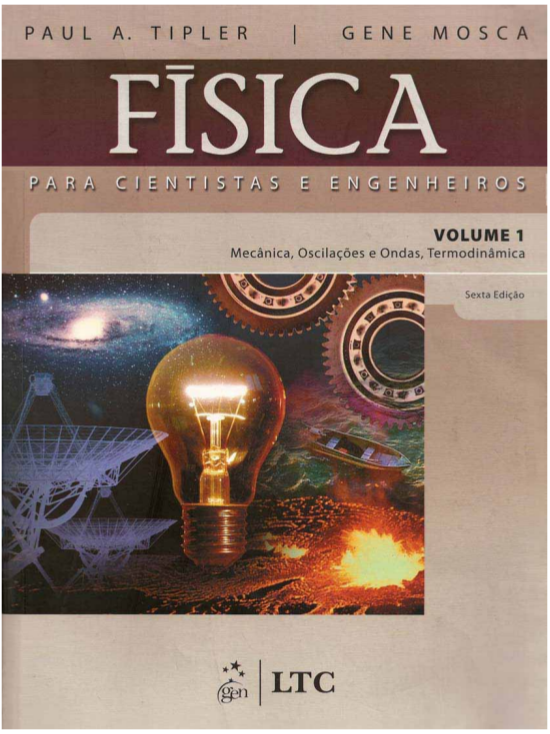
\includegraphics[height=\textheight-29pt]{images/tipler.png}
        };
    \end{tikzpicture}
\end{frame}

\newcommand{\NNotas}{3}
\begin{frame}{Avaliação}
    \begin{itemize}
        \item A avaliação será na forma de \NNotas{} notas: \(N_1\)\foreach \i in {2,...,\NNotas} {, \(N_\i\)}
        \item A média dos exercícios escolares (\(ME\)) será dada por
            \[
                    ME=\frac{N_1\foreach \i in {2,...,\NNotas} {+N_\i}}{\NNotas}
            \]
        \item Se \(ME \geq 8,0\), então a média final (\(MF\)) será igual à \(ME\)
        \item Se \(ME < 8,0\), então
            \[
                MF=\frac{2\times ME+PF}{3}
            \]
            onde PF é a nota da \textbf{prova final}
    \end{itemize}
\end{frame}


\section{Equilíbrio estático}

\begin{frame}{Força e torque}
    \begin{itemize}
        \item Forças causam variação no movimento \textbf{translacional}
        \item Torques causam variação no movimento \textbf{rotacional}
    \end{itemize}
    \begin{center}
        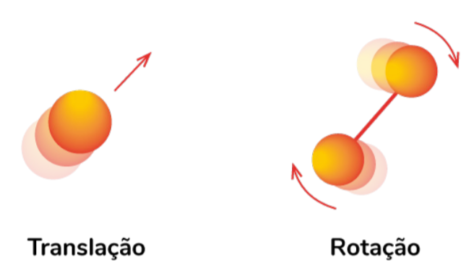
\includegraphics[width=6cm]{images/translação-rotação.png}
    \end{center}
    \pause
    Dessa forma, o que é necessário para que um corpo rígido esteja em \textbf{equilíbrio estático}?
\end{frame}

\begin{frame}{Equilíbrio estático}
    \begin{itemize}[<+->]
        \item A força externa resultante que atua sobre o corpo deve ser nula:
            \[
                \sum \vec{F}=\vec{0} \implies
                \begin{cases}
                    \sum F_x =0 \\ \sum F_y =0 \\ \textcolor{blue}{\sum F_z =0}
                \end{cases}
            \]

        \item O torque externo resultante deve ser nulo:
            \[
                \sum \vec{\tau}=\vec{0} \implies
                \begin{cases}
                    \textcolor{blue}{\sum \tau_x =0} \\
                    \textcolor{blue}{\sum \tau_y =0} \\
                    \sum \tau_z =0
                \end{cases}
            \]
    \end{itemize}
\end{frame}

\begin{frame}{Torque}
    \begin{itemize}
        \item Temos que
            \begin{align*}
                \vec{\tau} &= \vec{r} \times \vec{F} \\
                \tau &= r F \sen{\theta}
            \end{align*}
            onde \(\theta\) é o menor ângulo entre os vetores \(\vec{r}\) e \(\vec{F}\)
        \item Quando as forças e posições estão no \textbf{mesmo plano},
            a direção de \(\vec{\tau}\) é sempre perpendicular ao plano (''folha de papel''), mas o sentido depende da
            rotação que resultaria da ação do torque
            \begin{columns}
                \begin{column}{0.4\textwidth}
                    \begin{figure}
                        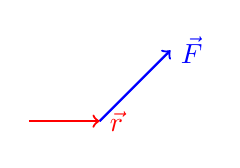
\begin{tikzpicture}[scale=0.45]
                            \draw [blue, thick, ->] (2,0) -- (4,2) node [right] { \(\vec{F}\) };
                            \draw [red, thick, ->] (0,0) -- (2,0) node [right] { \(\vec{r}\) };
                        \end{tikzpicture}
                        \caption{sentido positivo, saindo na folha de papel}
                    \end{figure}
                \end{column}

                \begin{column}{0.4\textwidth}
                    \begin{figure}
                        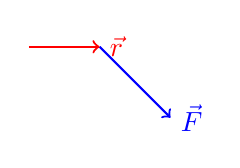
\begin{tikzpicture}[scale=0.45]
                            \draw [blue, thick, ->] (2,0) -- (4,-2) node [right] { \(\vec{F}\) };
                            \draw [red, thick, ->] (0,0) -- (2,0) node [right] { \(\vec{r}\) };
                        \end{tikzpicture}
                        \caption{sentido negativo, entrando da folha de papel}
                    \end{figure}
                \end{column}

            \end{columns}
    \end{itemize}
\end{frame}

\begin{frame}{''Os relógios são negativos...''}
    \centering
    \begin{tikzpicture}[scale=5]
        \draw[red,thick,->] (0,0,0) -- (1,0,0) node[below left]{$x$};
        \draw[blue, thick,->] (0,0,0) -- (0,1,0) node[below right]{$y$};
        \draw[black, thick,->] (0,0,0) -- (0,0,1) node[below right]{$z$};

        \only<1>{
        \draw[green!75!black, thick, ->] (0.5,0.5*tan{15}) arc (15:75:0.5/cos{15});
        \node [green!75!black, below] at (0.75,0.5) {rotação anti-horária};
        \draw [green!75!black,thick, ->] (0.3,0,0.25) -- (0.3,0,0.75) node [below] {sentido positivo};
    }
    \only<2>{
        \draw[magenta!75!black, thick, <-] (0.5,0.5*tan{15}) arc (15:75:0.5/cos{15});
        \node [magenta!75!black, below] at (0.75,0.5) {rotação horária};
        \draw [magenta!75!black,thick, ->] (0.3,0,0.75) node [below] {sentido negativo}-- (0.3,0,0.25);
    }
    \end{tikzpicture}
\end{frame}

\begin{frame}[c]{Vetores unitários e regra cíclica}
    \begin{columns}[T]
        \begin{column}{0.3\textwidth}
            \centering
            Sentido horário
            \begin{align*}
                \hat{i} \times \hat{j} & = \hat{k} \\
                \hat{j} \times \hat{k} & = \hat{i} \\
                \hat{k} \times \hat{i} & = \hat{j}
            \end{align*}
        \end{column}

        \begin{column}{0.3\textwidth}
            \centering
            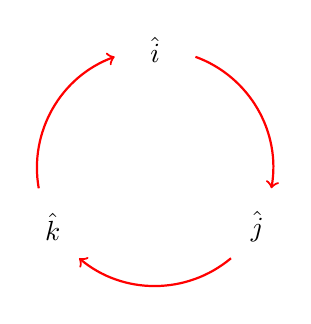
\begin{tikzpicture}[->,scale=1.5] 
                \foreach \a/\t in {90/i,-30/j,210/k}{
                    \node (\t) at (\a:1cm) {$\hat{\t}$};
                    \draw [thick,red] (\a-20:1cm) arc (\a-20:\a-100:1cm);
                } 
            \end{tikzpicture}

            \[
                \hat{i} \times \hat{i}  = \hat{j} \times \hat{j} = \hat{k} \times \hat{k} = \vec{0}
            \]

        \end{column}

        \begin{column}{0.3\textwidth}
            \centering
            Sentido anti-horário
            \begin{align*}
                \hat{i} \times \hat{k} & = -\hat{j} \\
                \hat{k} \times \hat{j} & = -\hat{i} \\
                \hat{j} \times \hat{i} & = -\hat{k}
            \end{align*}
        \end{column}
    \end{columns}
\end{frame}

\begin{frame}{Centro de massa}
    \begin{itemize}
        \item O centro de massa de um sistema de partículas é o ponto que se move como se (1) toda a massa do sistema estivesse
            concentrada nesse ponto e (2) todas as forças externas estivessem aplicadas nesse ponto
        \item Se o sistema de partículas é \textit{discreto}, temos
            \[
                \vec{r}_{CM} = \frac{1}{M} \sum_{i=1}^{N} m_i \vec{r}_i
            \]
        \item Se o sistema de partículas é \textit{contínuo}, temos
            \[
                \vec{r}_{CM} = \frac{1}{M} \int \vec{r}\; dm
            \]
    \end{itemize}
\end{frame}

\begin{frame}[c]{Centro de gravidade}
    \begin{itemize}
        \item A força gravitacional \( \vec{F}_g\) age \textit{efetivamente}
            sobre um único ponto de um corpo, o chamado \textbf{centro de
            gravidade} (CG) do corpo
    \item Se \( \vec{g}\) é igual para todos os elementos de um corpo, o centro
        de gravidade (CG) do corpo coincide com o centro de massa (CM)

    \item O torque devido a \(\vec{F}_g\) pode ser calculado como se
        \(\vec{F_g}\) estivesse aplicada \textit{somente} no centro de
            gravidade
    \end{itemize}
\end{frame}

\begin{frame}{Problemas do Halliday, capítulo 12}
    \includegraphics<1>[width=\textwidth]{images/Captura de tela de 2023-12-07 13-20-01.png}
    \includegraphics<1>[width=\textwidth-10pt*\real{3.72}]{images/Captura de tela de 2023-12-07 13-20-13.png}
    \includegraphics<1>[width=\textwidth]{images/Captura de tela de 2023-12-07 13-29-07.png}
\end{frame}

% \begin{frame}{Atividade 1}
%     \begin{itemize}
%         \item Vale 15\% da \(N_1\)
%         \item Grupo de no máximo 2 alunos\footnote{Pode ser individual}
%         \item Pode ser digitado ou manuscrito
%         \item Resolva os problemas 16, 35 e 41 do capítulo 12 do Halliday
%         \item Entrega no Google Sala de Aula até o dia 17/05
%     \end{itemize}
% \end{frame}

\begin{frame}{Problemas do Halliday, capítulo 12}
    \centering
    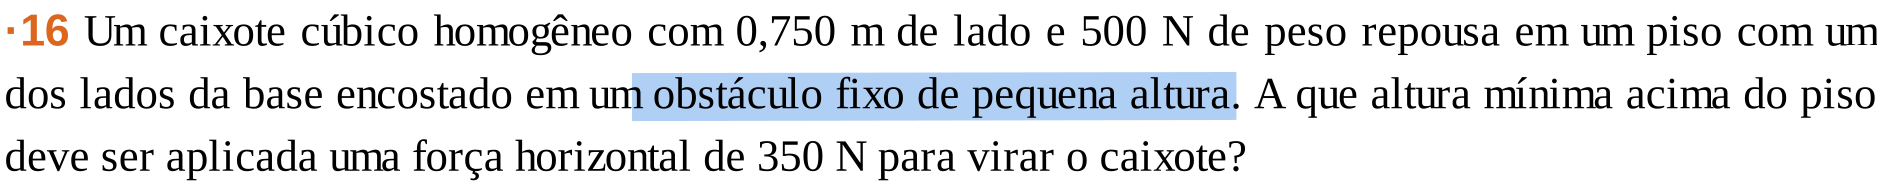
\includegraphics[width=\textwidth-4pt*\real{9.93}]{images/Captura de tela de 2023-12-07 12-56-58.png}
    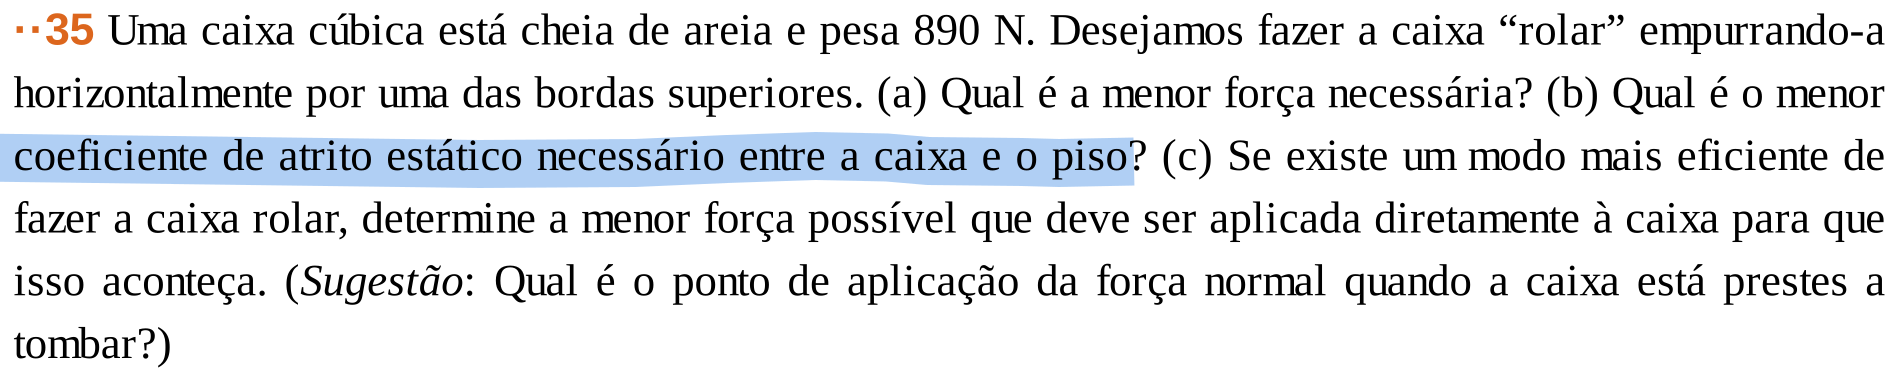
\includegraphics[width=\textwidth-4pt*\real{9.93}]{images/Captura de tela de 2023-12-07 13-38-29.png}
    % 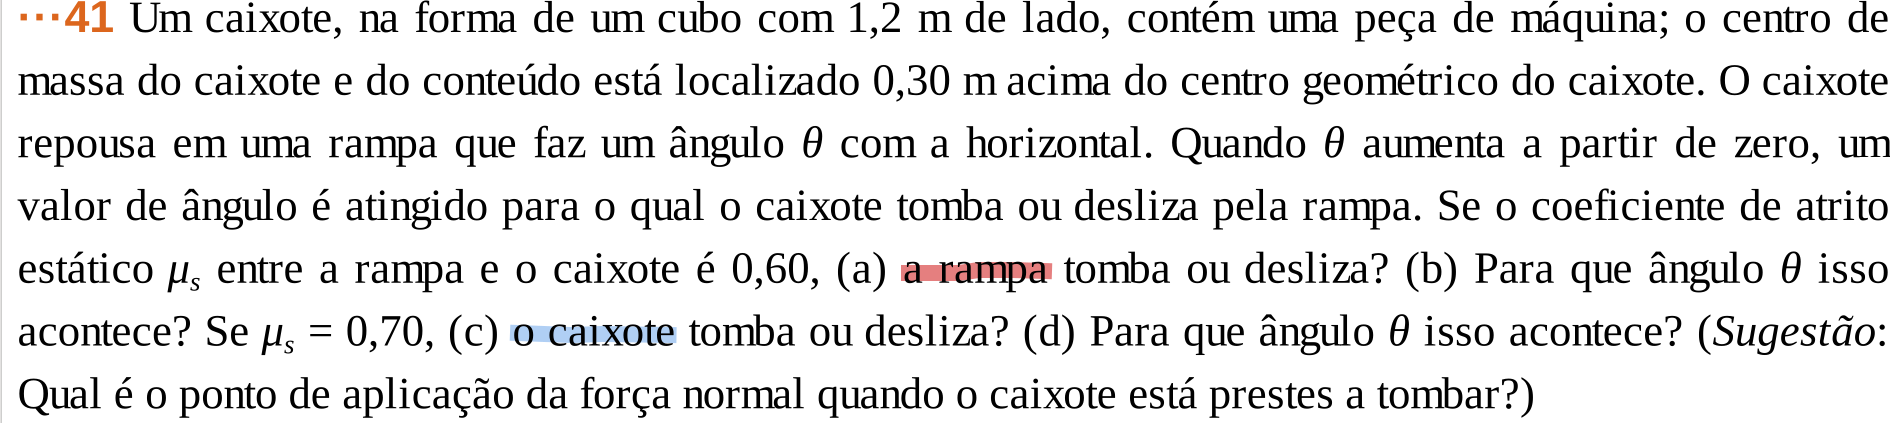
\includegraphics[width=\textwidth-4pt*\real{9.93}]{images/Captura de tela de 2023-12-07 12-57-51.png}
\end{frame}


\section{Fluidos}

\begin{frame}{Fluidos}
    \begin{itemize}
        \item Um fluido é uma substância que pode escoar, assumindo a forma do recipiente em que é colocado
        \item Quando discutimos corpos rígidos, as grandezas físicas que usamos são \textbf{massa} e \textbf{força}
            \begin{center}
                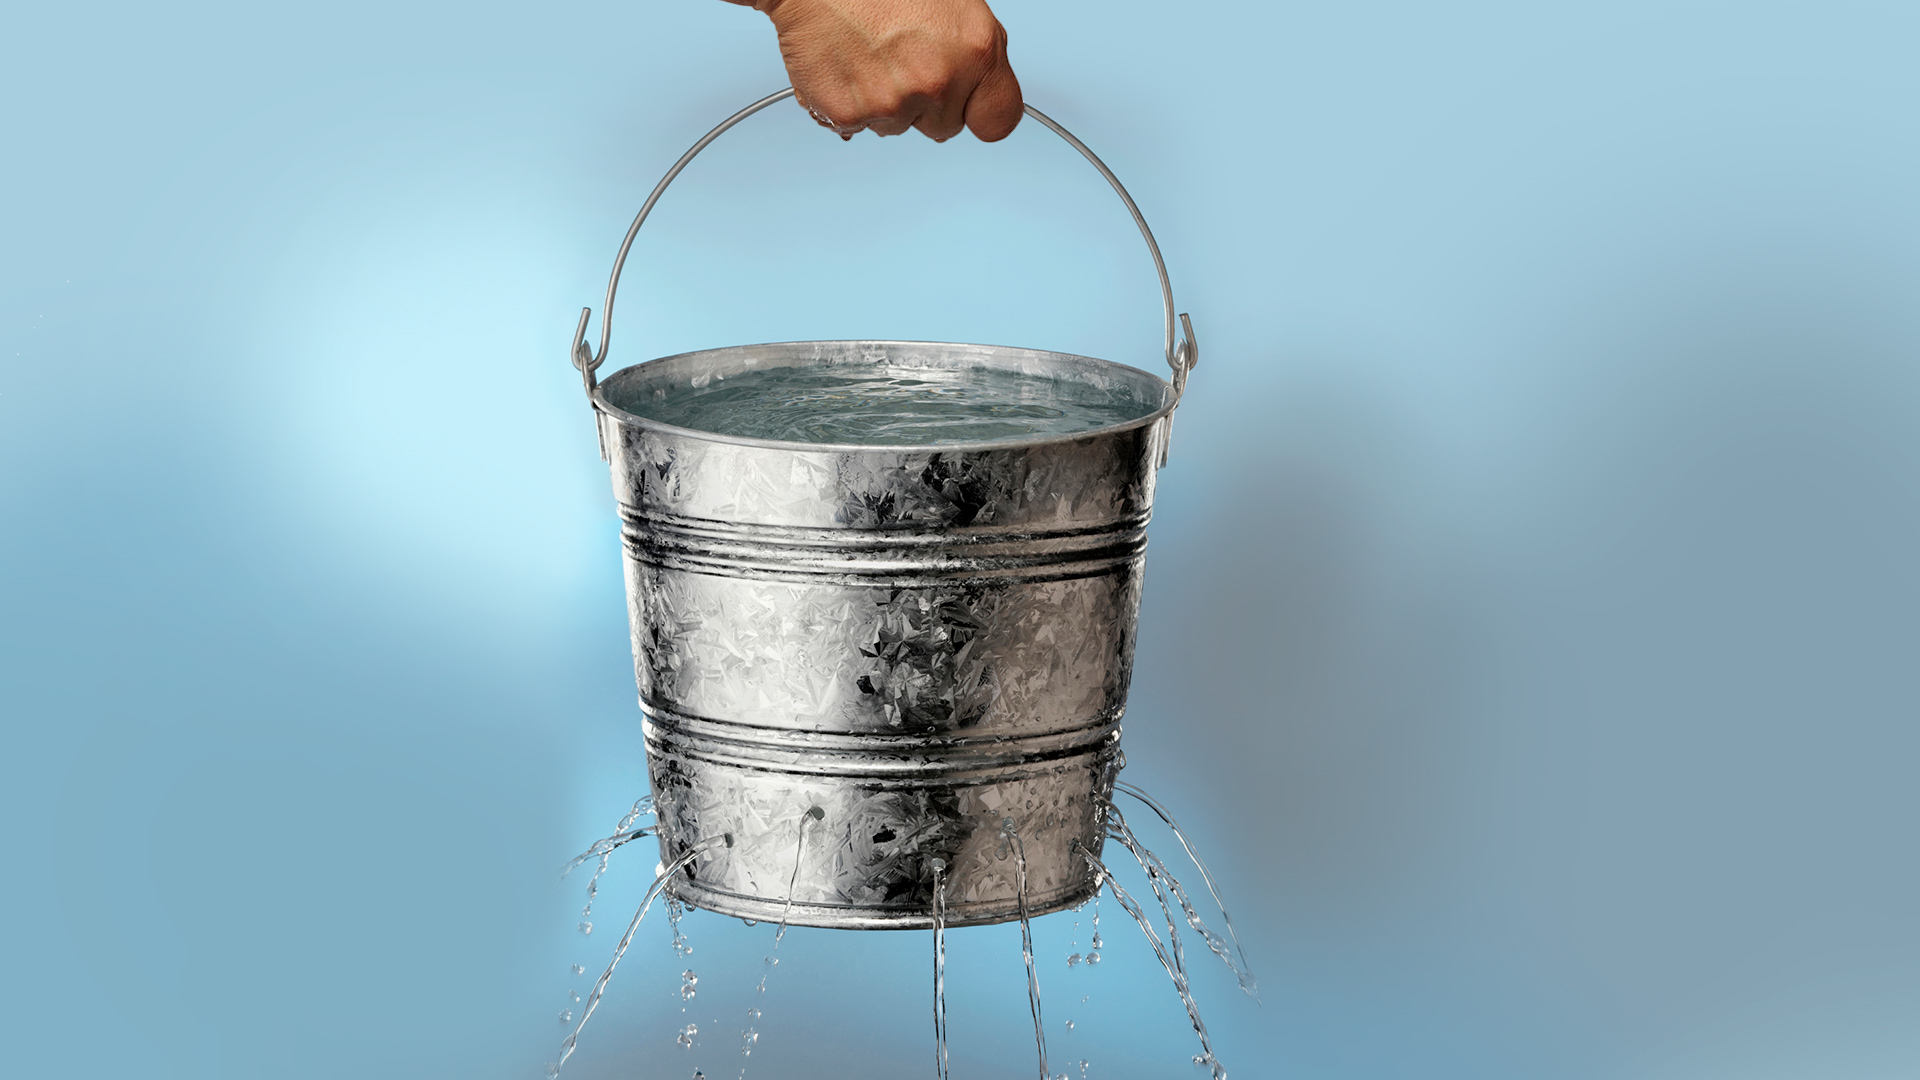
\includegraphics[width=0.6\textwidth]{images/balde_furado.jpg}
            \end{center}
        \item No caso de fluidos, é mais útil falar em \textbf{massa específica} e \textbf{pressão}
    \end{itemize}
\end{frame}

\begin{frame}{Algumas unidades...}
    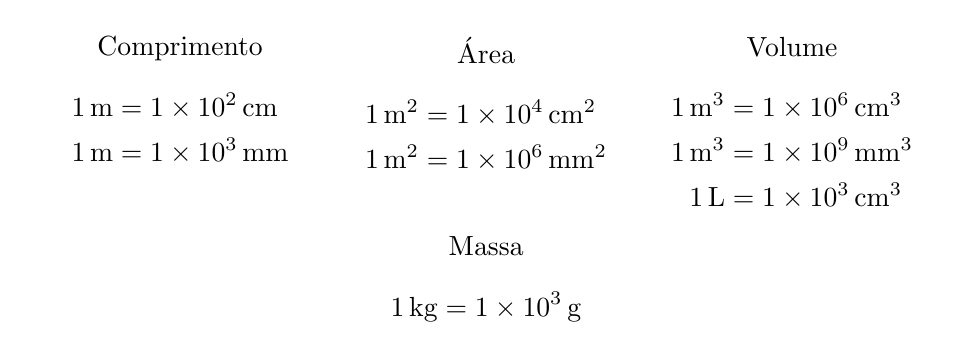
\begin{tikzpicture}
        \node [text width=0.3\textwidth] (Comprimento) at (0,0) {
            \centering
            Comprimento
            \begin{align*}
                \SI{1}{m} &= \SI{1e2}{cm} \\
                \SI{1}{m} &= \SI{1e3}{mm}
            \end{align*}
        };
        \node [text width=0.3\textwidth,anchor=north west] (Area) at (Comprimento.north east) {
            \centering
            Área
            \begin{align*}
                \SI{1}{m^2} &= \SI{1e4}{cm^2} \\
                \SI{1}{m^2} &= \SI{1e6}{mm^2}
            \end{align*}
        };
        \node [text width=0.3\textwidth,anchor=north west] (Volume) at (Area.north east) {
            \centering
            Volume
            \begin{align*}
                \SI{1}{m^3} &= \SI{1e6}{cm^3} \\
                \SI{1}{m^3} &= \SI{1e9}{mm^3} \\
                \SI{1}{L} &= \SI{1e3}{cm^3}
            \end{align*}
        };
        \node [text width=0.3\textwidth,anchor=north west] (Massa) at (Area.south west |- Volume.south west) {
            \centering
            Massa
            \begin{align*}
                \SI{1}{kg} &= \SI{1e3}{g}
            \end{align*}
        };
    \end{tikzpicture}

    \vspace{3cm-12pt}
    \pause
    Qual a relação entre \(\si{g/cm^3}\) e \(\si{kg/m^3}\)?
\end{frame}

\begin{frame}{Massa específica}
    \begin{itemize}
        \item A massa específica média de um corpo é dada por:
            \[
                \bar{\rho} = \frac{\Delta  m}{\Delta V}
            \]

        \item A massa específica de um ponto qualquer de um corpo é:
            \[
                \rho = \frac{dm}{dV}
            \]
        \item Para um corpo uniforme $\rho = \bar{\rho}$

        \item A unidade SI para a massa específica é o $\si{kg/m^3}$
    \end{itemize}

\end{frame}

\begin{frame}{Pressão}

    \begin{itemize}
        \item A pressão $P$ sobre uma superfície é força por unidade de área:
            \[
                P=\frac{F}{A}
            \]
            onde $F$ é o módulo da força \textbf{normal à superfície} e $A$ é a área da superfície
        \item A pressão é uma grandeza \textbf{escalar} de onde podemos obter uma grandeza \textbf{vetorial} (força)

        \item Se a pressão \textbf{varia} sobre uma área, a força infinitesimal
            $dF$ sobre um elemento de superfície infinitesimal de área $dA$ é:
            \[
                dF=P dA
            \]
        \item A unidade SI para a pressão é o pascal: $\SI{1}{Pa} = \SI{1}{N/m^2}$
    \end{itemize}
\end{frame}

\begin{frame}{Outras unidades de pressão}
    Além do pascal, também são comumente usadas:
    \begin{itemize}
        \item \SI{1}{bar} = \SI{100}{kPa}\
        \item \SI{1}{psi} = \(\SI{1}{lbf/in^2}\) = \(\displaystyle \frac{\SI{4.4482}{N}}{(\SI{0.0254}{m})^2}\) = \SI{6894.7548}{Pa}
        \item \SI{1}{atm} = \SI{101.325}{kPa} = \SI{14.7}{psi}
        \item \SI{760}{mmHg} = \SI{1}{atm}
    \end{itemize}
    \centering
    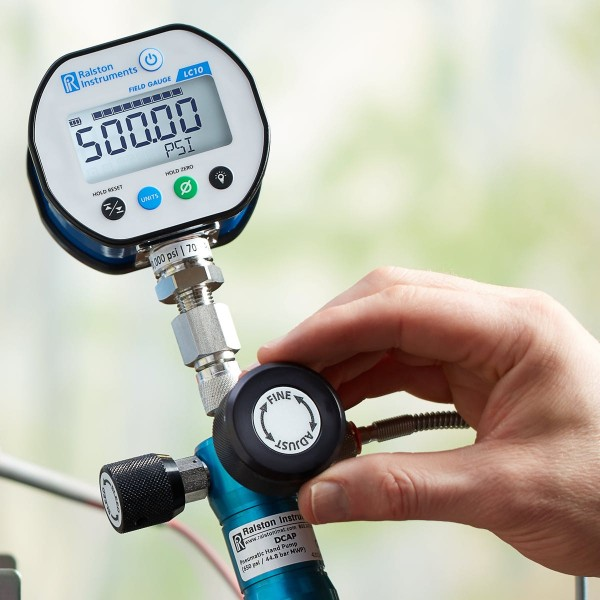
\includegraphics[height=\textheight-106pt]{images/manometro-digital-medidor-de-pressao-digital-lc10-1-600x600.jpg}
    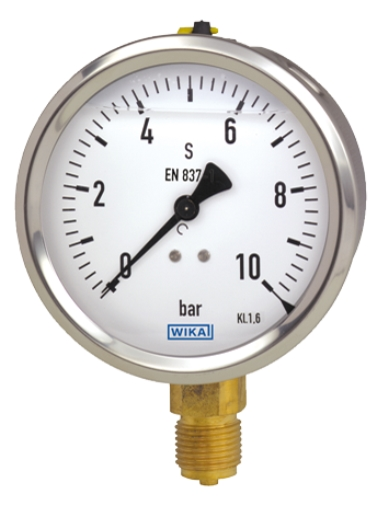
\includegraphics[height=\textheight-106pt]{images/213.53.jpg}
    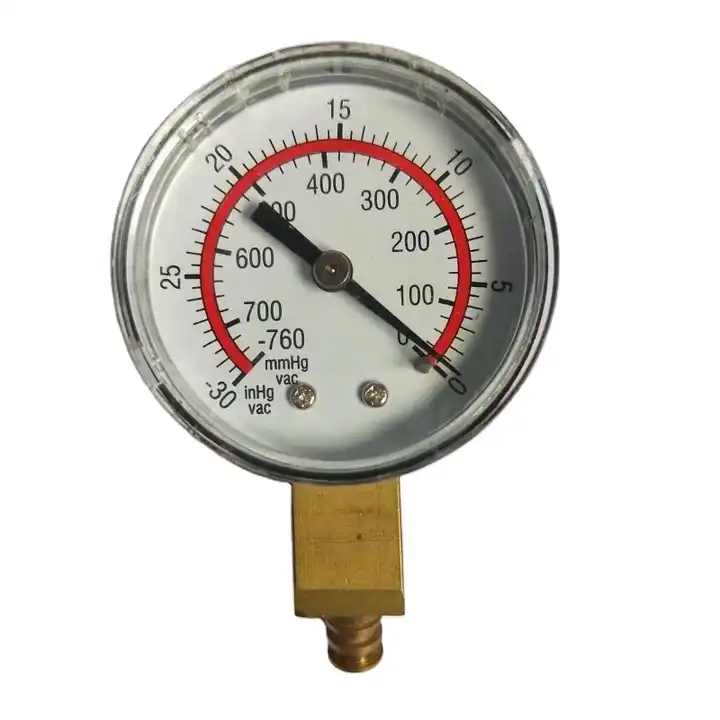
\includegraphics[height=\textheight-106pt]{images/mmHg.png}
\end{frame}

\begin{frame}{Problema 1 do Halliday, capítulo 14}
    \begin{minipage}{\textwidth}
        Um peixe se mantém na mesma profundidade na água doce ajustando a quantidade
        de ar em ossos porosos ou em bolsas de ar para tornar sua massa específica média
        igual à da água. Suponha que, com as bolsas de ar vazias, um peixe tem uma massa
        específica de \(\SI{1,08}{g/cm^3}\). Para que fração de seu novo volume o peixe deve inflar
        as bolsas de ar para tornar sua massa específica igual à da água?
    \end{minipage}

    \vspace{1cm}
    \textit{Dados:}
    \begin{itemize}
        \item Massa específica da água: \(\SI{1,00}{g/cm^3}\)
    \end{itemize}
\end{frame}

\begin{frame}{Problemas do Halliday, capítulo 14}
    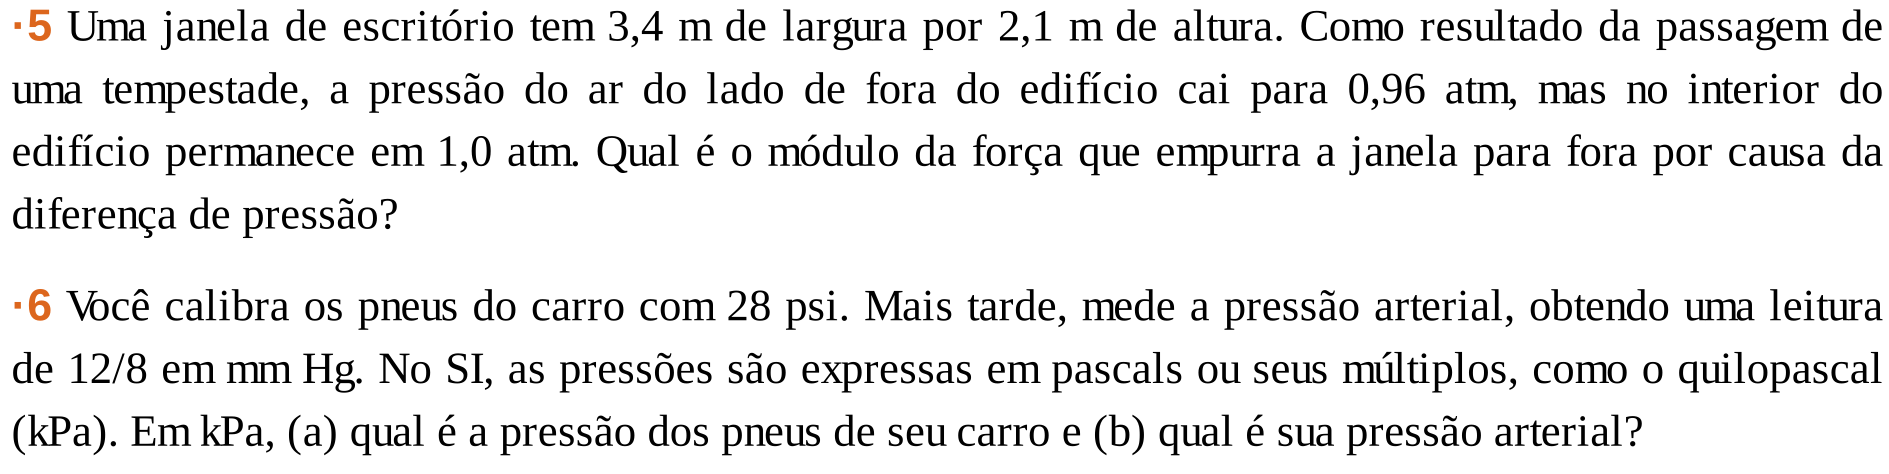
\includegraphics[width=\textwidth]{images/Captura de tela de 2024-01-11 14-52-09.png}
\end{frame}

\begin{frame}{Pressão em Fluidos}
    \begin{itemize}
        \item A pressão em um fluido aumenta com a profundidade
        \item A pressão em um fluido \textbf{incompressível} aumenta \textbf{linearmente} com a profundidade
            \[
                P=P_0 + \rho g h
            \]
        \item \textbf{Princípio de Pascal}: Variações de pressão aplicadas em
            um fluido \textbf{incompressível} confinado são transmitidas, sem
            redução, a todos os pontos do fluido e às paredes do recipiente
            \[
                \Delta P_1 = \Delta P_2 = \ldots = \Delta P_n
            \]
    \end{itemize}
\end{frame}

\begin{frame}{Problema 10 do Halliday, capítulo 14}
    \begin{minipage}{\textwidth}
        O tubo de plástico da figura abaixo tem uma seção reta de \(\SI{5,00}{cm^2}\).
        Introduz-se água no tubo até o lado mais curto (de comprimento \(d= \SI{0,800}{m}\) fique
        cheio. Em seguida, o lado menor é fechado e mais água é despejada no lado maior. Se a tampa do lado menor
        é arrancada quando a força a que está submetida excede \SI{9,80}{N}, que altura da coluna de água do lado
        maior deixa a tampa na iminência de ser arrancada?
    \end{minipage}

    \vspace{1cm}\centering
    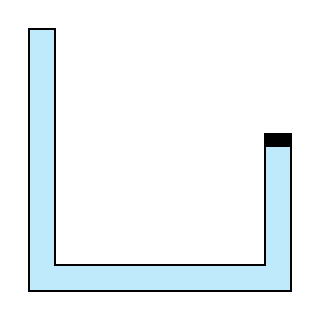
\begin{tikzpicture}[scale=1/3]
        \draw [thick, fill=cyan!25] (0,10) -- (0,0) -- (10,0) -- (10,6) --  (9,6) -- (9,1) -- (1,1) -- (1,10) -- cycle;
        \filldraw [black] (9,6) rectangle (10,5.5);
    \end{tikzpicture}
\end{frame}

\begin{frame}{Problemas do Halliday, capítulo 14}
    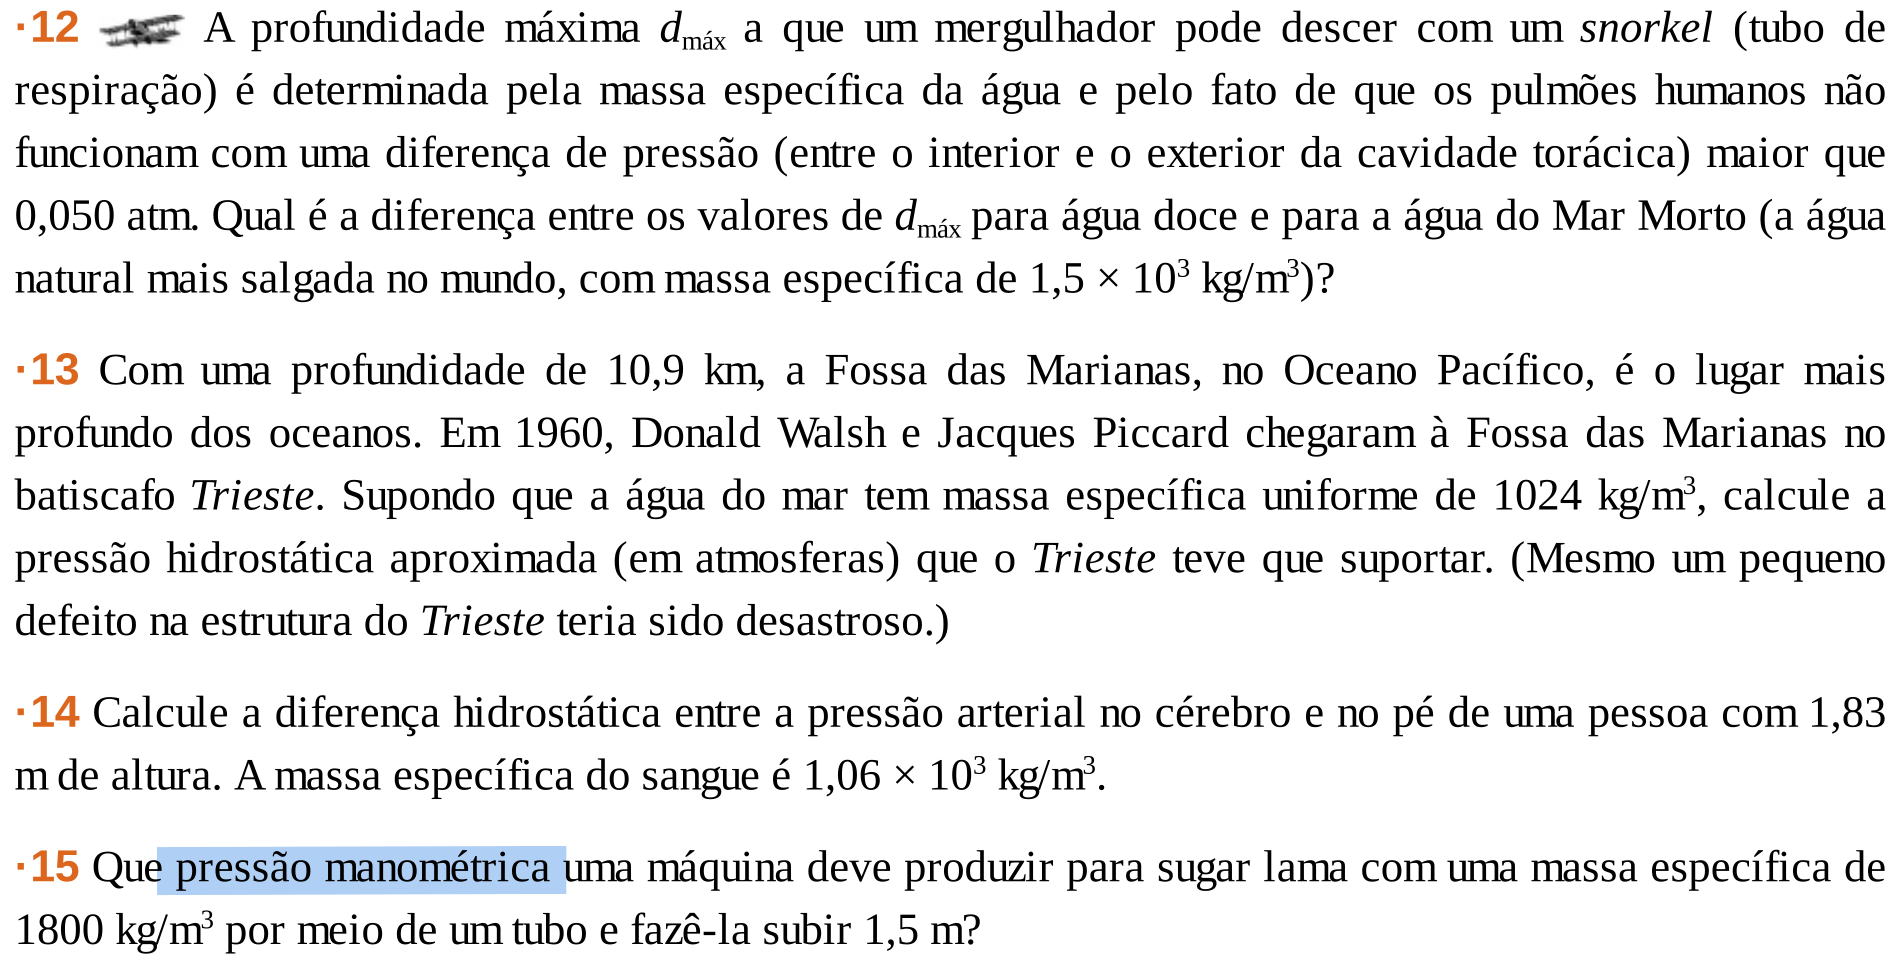
\includegraphics[height=\textheight-28pt]{images/Captura de tela de 2024-01-11 14-57-52.png}
\end{frame}

\begin{frame}{Princípio de Arquimedes}
    Um corpo total ou parcialmente mergulhado em um fluido sofre uma \textbf{força
    de empuxo} vertical de baixo para cima igual ao peso do fluido por ele
    deslocado:
    \[E=\rho g V_{sub}\]

    \begin{center}
        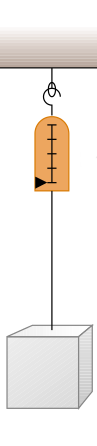
\includegraphics[height=0.4\textheight]{images/empuxo1}
        \hspace*{1cm}
        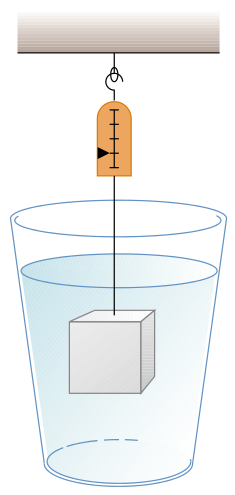
\includegraphics[height=0.4\textheight]{images/empuxo2}
    \end{center}

    O peso aparente $F_{ap}$ de um corpo imerso em um fluido é a diferença entre os
    módulos do seu peso $F_{g}$ e do empuxo $E$: \[F_{ap}=F_{g}-E\]
\end{frame}

\begin{frame}{Problemas do Halliday, capítulo 14}
    \centering
    \includegraphics<+>[height=\textheight-28pt]{images/Captura de tela de 2024-01-23 12-13-05.png}

    \includegraphics<+>[width=\textwidth]{images/Captura de tela de 2024-01-23 12-23-46.png}
\end{frame}

\begin{frame}{Fluidos em movimento}
    Até agora nosso estudo foi restrito a fluidos em repouso. Quando um fluido está
    em movimento, o fluxo pode ser caracterizado como sendo:

    \begin{itemize}
        \item regular ou laminar: cada partícula do fluido segue uma trajetória reta de
            forma que as trajetórias de diferentes partículas nunca se cruzem.

        \item turbulento: as trajetórias das partículas formam redemoinhos em algumas
            regiões.
    \end{itemize}
    \centering
    \adjincludegraphics[width=0.45\textwidth+8pt/\real{1.35},trim={0 {0.5\height+8pt} 0 0},clip]{images/laminar_vs_turbulento.png}
    \adjincludegraphics[width=0.45\textwidth-8pt/\real{1.35},trim={0 0 0 {0.5\height-8pt}},clip]{images/laminar_vs_turbulento.png}

    \begin{block}<+->{Observação}
    Quando a velocidade de escoamento de um fluido se torna suficientemente grande,
    o escoamento deixa de ser laminar e se torna turbulento.
    \end{block}
\end{frame}

\begin{frame}{Vazão}
    \begin{itemize}
        \item Na figura, o fluido escoa da esquerda para direita sem turbulência
        \item A massa $\Delta m_1$ que escoa através da superfície 1 é dada por:
    \end{itemize}
    \[
        \Delta m_1 = \rho_1 \Delta V_1 = \rho_1 A_1 \Delta x_1 = \rho_1 A_1 v_1 \Delta t
    \]
    \begin{center}
        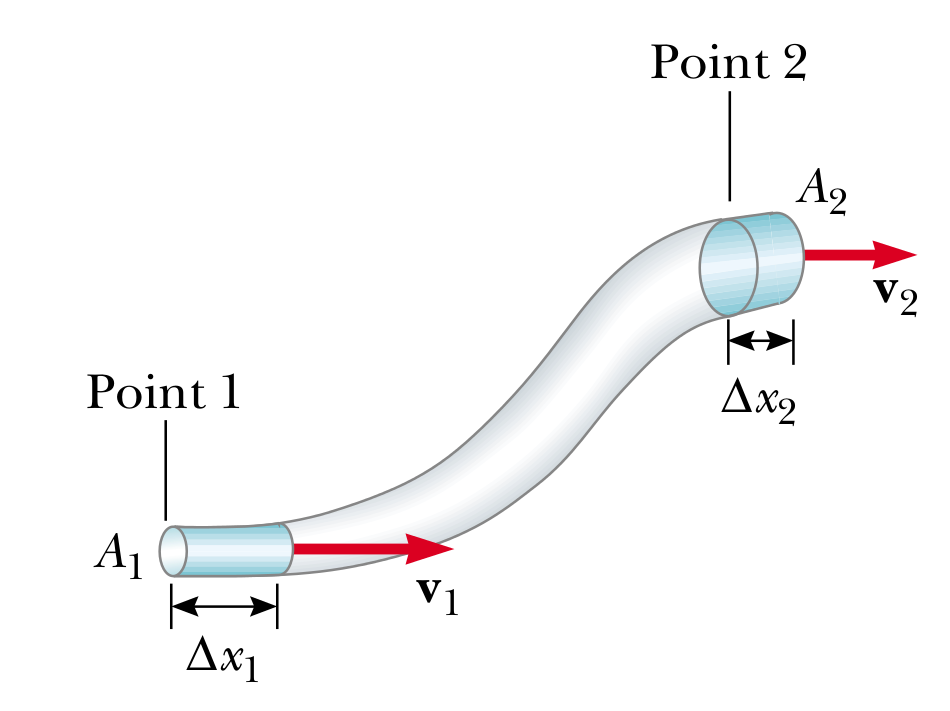
\includegraphics[width=0.45\textwidth]{images/tuboS}
    \end{center}
\end{frame}

\begin{frame}
    \begin{itemize}
        \item A quantidade $I_M=\rho A v$ é chamada de \textbf{vazão mássica}
        \item As dimensões de $I_M$ são as de massa dividida por tempo
        \item A massa que atravessa a superfície 2 durante o mesmo tempo $\Delta t$ é:
    \end{itemize}
    \[
        \Delta m_2 = \rho_2 A_2 v_2 \Delta t
    \]
    \begin{center}
        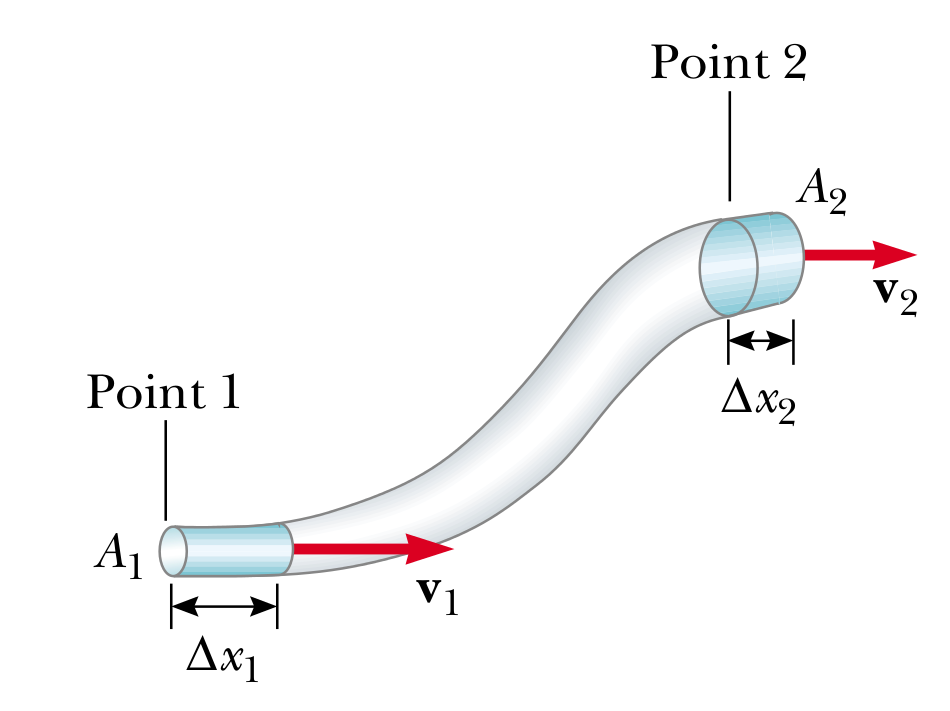
\includegraphics[width=0.45\textwidth]{images/tuboS}
    \end{center}
\end{frame}

\begin{frame}[c]
    A diferença entre a taxa na qual massa entra no tubo e a taxa na qual a massa
    sai do tubo é igual a taxa de variação da massa do tubo:
    \[
        \frac{\Delta m_1}{\Delta t} - \frac{\Delta m_2}{\Delta t} = \frac{dm}{dt} ~\rightarrow~ I_{M1}-I_{M2} = \frac{dm}{dt}
    \]
    essa equação é chamada de \textbf{equação da continuidade}.
\end{frame}

\begin{frame}
    Escoamento no qual o movimento do fluido é constante (não varia com o tempo) em
    todos os pontos é chamado \textbf{estacionário}. Em um escoamento estacionário
    a vazão mássica em um dado instante é a mesma através de todas as superfícies
    de seção reta. Além disso, a vazão mássica é constante.

    \[
        \frac{dm}{dt}=0 ~\rightarrow~ I_{M1}=I_{M2}
    \]

    A quantidade $I_V = Av$ é chamada de \textbf{vazão volumétrica}. Para um fluido incompressível, temos:
    \[
        I_{V1}=I_{V2}
    \]
\end{frame}

\begin{frame}<1>[label=tora]{Problemas do Halliday, capítulo 14}
    \centering
    \includegraphics<+>[width=\textwidth]{images/Captura de tela de 2024-05-14 16-29-06.png}

    \includegraphics<.>[height=(\textheight-116pt)*\real{0.64}]{images/Captura de tela de 2024-05-14 16-30-02.png}

    \includegraphics<+>[width=\textwidth]{images/Captura de tela de 2024-05-14 16-38-05.png}
\end{frame}

% \begin{frame}{Problema do Tipler, capítulo 13}
%     \centering
%     \includegraphics<+->[width=\textwidth]{images/Captura de tela de 2024-05-14 16-48-49.png}

%     \vspace{2cm-30pt}

%     \includegraphics<+>[width=\textwidth]{images/Captura de tela de 2024-05-14 16-56-52.png}

%     \only<.>{\textbf{(Figura que não faz parte do enunciado do problema)}}
% \end{frame}

% \againframe<2->{tora}

\begin{frame}{Atividade}
    \begin{itemize}
        \item Vale 25\% da \(N_1\)
        \item Grupo de no máximo 2 alunos\footnote{Pode ser feito individualmente}
        \item Pode ser digitado ou manuscrito
        \item Fazer uma pesquisa sobre \textit{Equação de Bernoulli}
        \item Entrega até o dia 17/5 na Sala de Aula
    \end{itemize}

    \centering\url{https://classroom.google.com/c/NzcyMzIxOTQ4NzQx?cjc=dwqjunh7}
\end{frame}

% \begin{frame}{Equação de Bernoulli}
%     A equação de Bernoulli relaciona a pressão, a altura e a velocidade (módulo) de
%     um fluido \textbf{incompressível não-viscoso em escoamento estacionário}:
%     \[
%         P_2+\rho g h_2 + \frac{1}{2}\rho v^2_2 = P_1+\rho g h_1 + \frac{1}{2}\rho v^2_1
%     \]

%     A equação de Bernoulli pode ser enunciada, também, como
%     \[
%         P+\rho g h + \frac{1}{2}\rho v^2 = \mathrm{constante}
%     \]

%     Para um fluido em repouso, temos:
%     \[
%         P+\rho g h = \mathrm{constante}
%     \]
% \end{frame}

% \begin{frame}{Problemas do Halliday, capítulo 14}
%     \centering
%     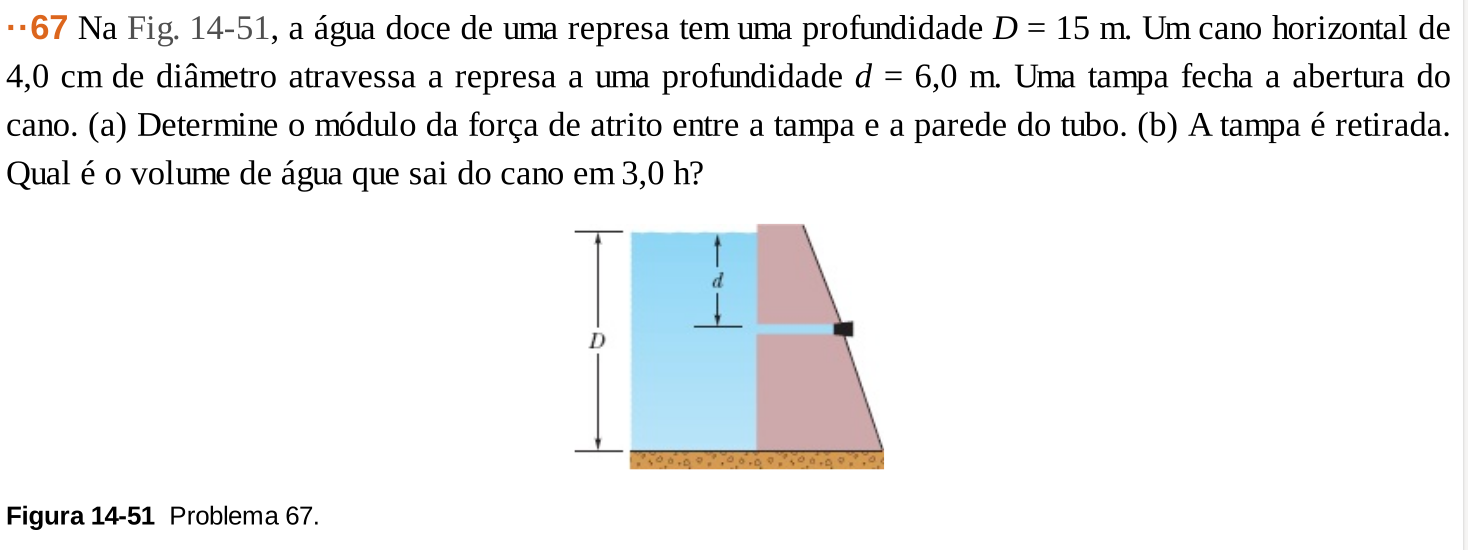
\includegraphics[width=\textwidth]{images/Captura de tela de 2025-04-09 10-25-00.png}
% \end{frame}

% \begin{frame}{Problemas do Halliday, capítulo 14}
%     \centering
%     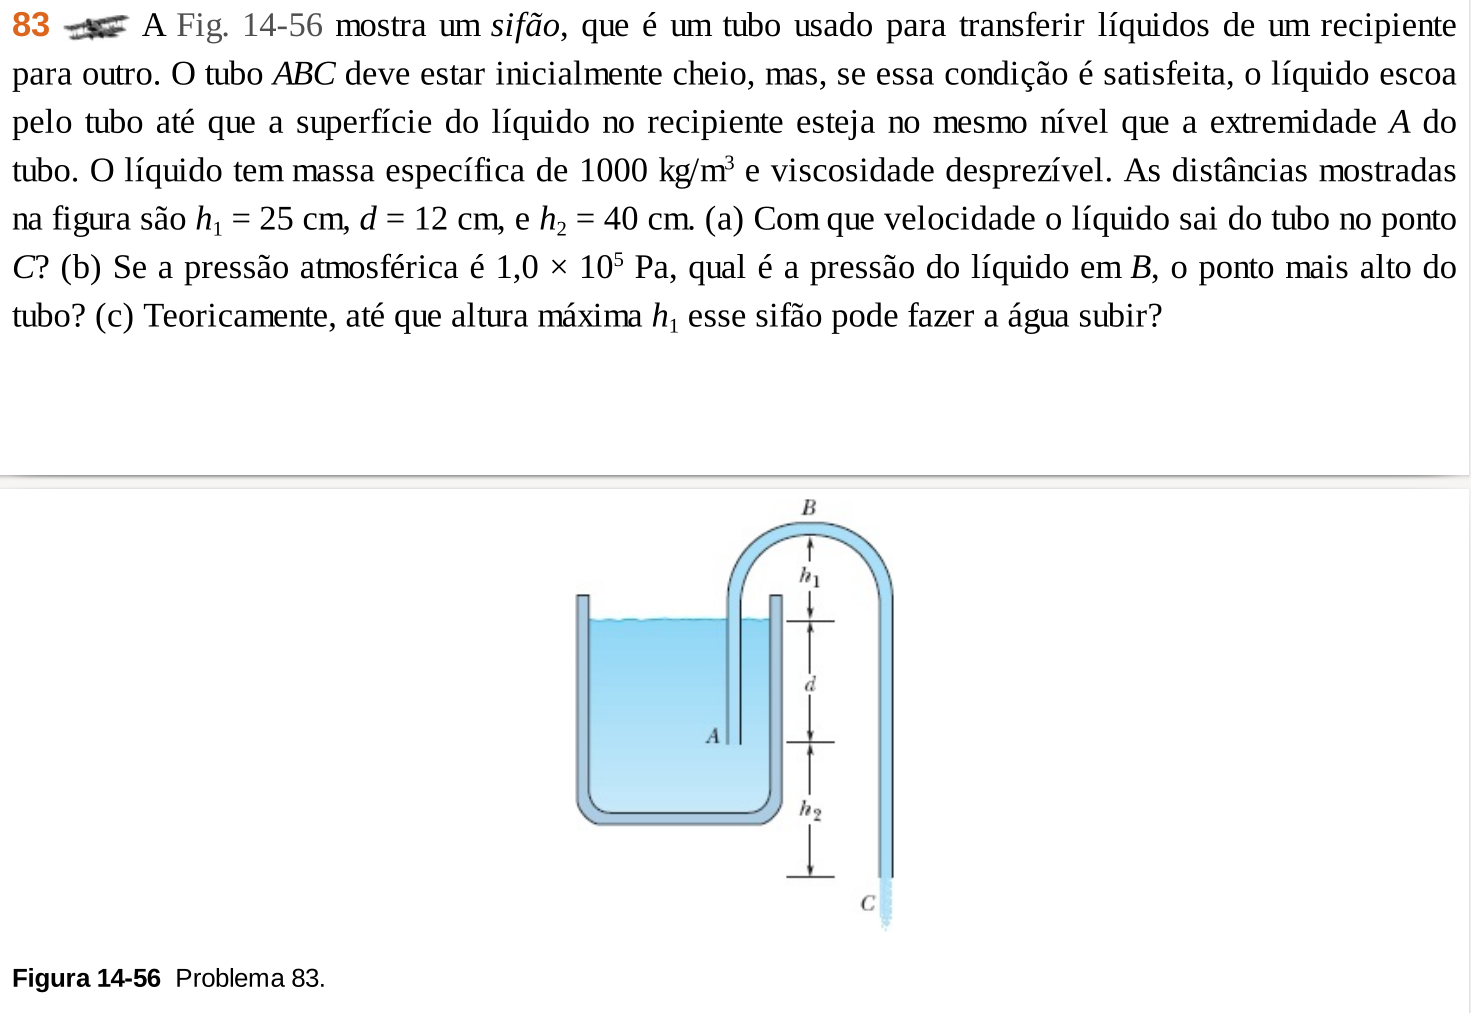
\includegraphics[height=\textheight-28pt]{images/Captura de tela de 2025-04-09 10-23-22.png}
% \end{frame}


% \begin{frame}{Segunda lista de exercícios para a prova 1}
%     \begin{itemize}
%         \item Problemas 1, 5, 6, 10, 12, 13, 14, 15, 18, 31, 32, 33, 44, 45, 46
%             e 48 do capítulo 14
%         \item \textit{Pelo menos} dois desses problemas cairão na prova
%     \end{itemize}
% \end{frame}

% \begin{frame}[c]
%     \centering
%     Fim do assunto para a primeira prova
% \end{frame}


\section{Oscilações e ondas}

\begin{frame}{Oscilações -- Lei de Hooke}
    \begin{center}
        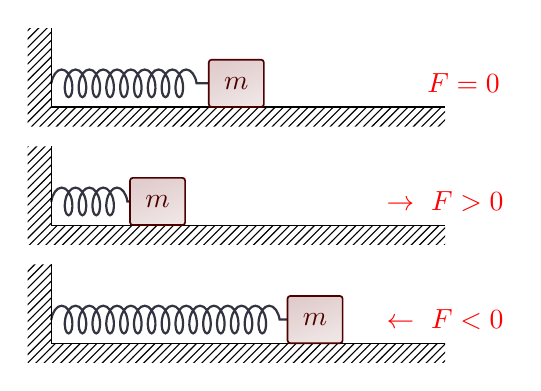
\begin{tikzpicture}[
            ground/.style={fill,pattern=north east lines,draw=none,minimum width=0.3,minimum height=0.6},
            spring/.style={line width=0.8,blue!7!black!80,decorate, decoration={coil,amplitude=5,segment length=5},line cap=round},
            mass/.style={line width=0.6,red!30!black,fill=red!40!black!10,rounded corners=1,
            top color=red!40!black!20,bottom color=red!40!black!10,shading angle=20}
            ]
            \def\H{1}    % wall height
            \def\T{0.3}  % wall thickness
            \def\W{5.0}  % ground length
            \def\D{0.25} % ground depth
            \def\h{0.6}  % mass height
            \def\w{0.7}  % mass width
            \def\x{1.6}  % mass x position

            \foreach \y/\x in {0/2.0,1.5/1.0,3/3.0} {
                \begin{scope}[shift={(0,-\y)}]
                    \draw[spring] (0,\h/2) --++ (\x,0);
                    \draw[ground] (0,0) |-++ (-\T,\H) |-++ (\T+\W,-\H-\D) -- (\W,0) -- cycle;
                    \draw (0,\H) -- (0,0) -- (\W,0);
                    \draw[mass] (\x,0) rectangle++ (\w,\h) node[midway] {$m$};
                \end{scope}
            }
            \node [red] at (\W,\h/2) {$\phantom{\rightarrow~}F=0$};
            \node [red] at (\W,\h/2-1.5) {$\rightarrow~F>0$};
            \node [red] at (\W,\h/2-3) {$\leftarrow~F<0$};
        \end{tikzpicture}
    \end{center}

    \[
        F = -kx \rightarrow
        \begin{cases}
            F = 0, \text{ se } x =0\\
            F > 0, \text{ se } x<0\\
            F < 0, \text{ se } x>0
        \end{cases}
        \rightarrow
        \text{Força restauradora}
    \]
\end{frame}

\begin{frame}{Equação diferencial}
    \[
        F=-kx \implies ma=-kx \implies m\frac{d^2 x}{dt^2}=-kx \implies \frac{d^2 x}{dt^2}=-\frac{k}{m} x
    \]
    \begin{gather*}
    \Downarrow \\
    \boxed{\color{blue} \frac{d^2 u}{dt^2}= -\omega^2 u \implies \text{Movimento Harmônico Simples}}
    \end{gather*}
    Solução geral:
    \[
        u=C_1 \sen{\omega t} + C_2 \cos{\omega t} \implies
        \begin{cases}
            A \sin{(\omega t + \delta)} \\
            A \cos{(\omega t + \delta)}
        \end{cases}
        \implies A \cos{(\omega t + \delta)}
    \]
\end{frame}

\begin{frame}{Gráfico de \(u=A \cos{(\omega t+\delta)}\)}
    \begin{columns}[c]
        \begin{column}{0.6\textwidth}
            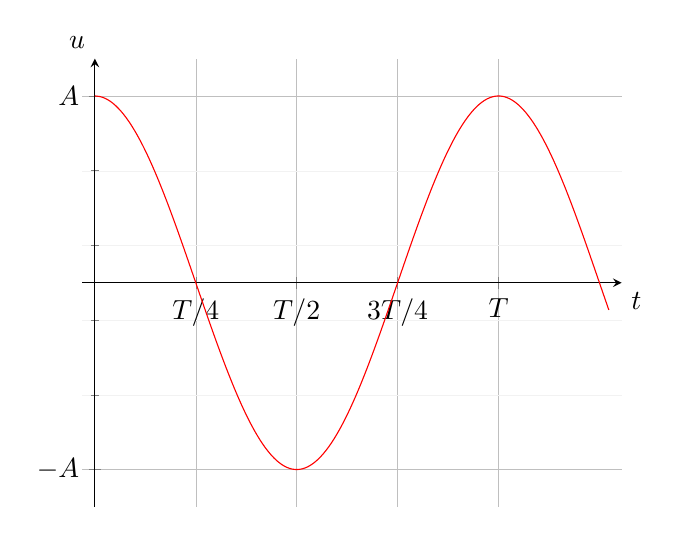
\begin{tikzpicture}
                \begin{axis}%
                    [grid=both,
                    minor tick num=4,
                    grid style={line width=.1pt, draw=gray!10},
                    major grid style={line width=.2pt,draw=gray!50},
                    axis lines=middle,
                    enlargelimits={abs=0.2},
                    xlabel={$t$},
                    ylabel={$u$},
                    xlabel style={below right},
                    ylabel style={above left},
                    xtick={pi/2,pi,3*pi/2, 2*pi},
                    xticklabels={$T/4$,$T/2$,$3T/4$,$T$},
                    ytick={-1,1},
                    yticklabels={$-A$,$A$}
                    ]
                    \addplot[domain=0:8,samples=100,smooth,red] {cos(deg(x))};
                \end{axis}
            \end{tikzpicture}
        \end{column}

        \begin{column}{0.4\textwidth}
            \begin{itemize}
                \item \(A\) é a amplitude
                \item \(T\) é o período e \(T=2\pi/\omega\)
                \item \(\omega t + \delta\) é a fase
                \item \(\delta\) é a constante de fase
                \item \(\omega\) é a frequência angular
                \item \(f\) é a frequência e \(\omega = 2\pi f\)
                    \[
                        \color{blue}
                        T=\frac{1}{f}
                    \]
            \end{itemize}
            \begin{tcolorbox}[colback=blue!10]
                No SI, T é em \si{s}, \(\omega\) é em \si{rad/s} e f é em \si{Hz} (ciclo/s)
            \end{tcolorbox}
        \end{column}
    \end{columns}
\end{frame}

\begin{frame}{Problemas do Halliday, capítulo 15}
    \centering
    \includegraphics<+>[width=\textwidth]{images/Captura de tela de 2024-01-25 13-27-30.png}

    \includegraphics<+>[width=\textwidth]{images/Captura de tela de 2024-01-25 13-28-14.png}
\end{frame}

\begin{frame}{A constante de fase}
    \centering
    \begin{columns}[c]
        \begin{column}{0.45\textwidth}
            \[\delta = 0\]
            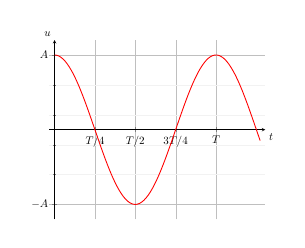
\begin{tikzpicture}[scale=0.4]
                \begin{axis}%
                    [grid=both,
                    minor tick num=4,
                    grid style={line width=.1pt, draw=gray!10},
                    major grid style={line width=.2pt,draw=gray!50},
                    axis lines=middle,
                    enlargelimits={abs=0.2},
                    xlabel={$t$},
                    ylabel={$u$},
                    xlabel style={below right},
                    ylabel style={above left},
                    xtick={pi/2,pi,3*pi/2, 2*pi},
                    xticklabels={$T/4$,$T/2$,$3T/4$,$T$},
                    ytick={-1,1},
                    yticklabels={$-A$,$A$}
                    ]
                    \addplot[domain=0:8,samples=100,smooth,red,thick] {cos(deg(x))};
                \end{axis}
            \end{tikzpicture}

            \[\delta = \pi\]
            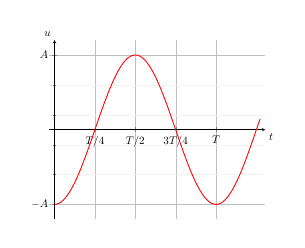
\begin{tikzpicture}[scale=0.4]
                \begin{axis}%
                    [grid=both,
                    minor tick num=4,
                    grid style={line width=.1pt, draw=gray!10},
                    major grid style={line width=.2pt,draw=gray!50},
                    axis lines=middle,
                    enlargelimits={abs=0.2},
                    xlabel={$t$},
                    ylabel={$u$},
                    xlabel style={below right},
                    ylabel style={above left},
                    xtick={pi/2,pi,3*pi/2, 2*pi},
                    xticklabels={$T/4$,$T/2$,$3T/4$,$T$},
                    ytick={-1,1},
                    yticklabels={$-A$,$A$}
                    ]
                    \addplot[domain=0:8,samples=100,smooth,red,thick] {cos(deg(x+pi))};
                \end{axis}
            \end{tikzpicture}
        \end{column}

        \begin{column}{0.45\textwidth}
            \[\delta = \pi/2\]
            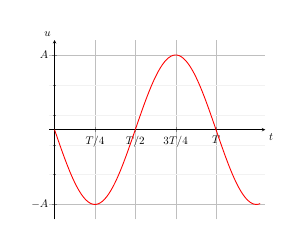
\begin{tikzpicture}[scale=0.4]
                \begin{axis}%
                    [grid=both,
                    minor tick num=4,
                    grid style={line width=.1pt, draw=gray!10},
                    major grid style={line width=.2pt,draw=gray!50},
                    axis lines=middle,
                    enlargelimits={abs=0.2},
                    xlabel={$t$},
                    ylabel={$u$},
                    xlabel style={below right},
                    ylabel style={above left},
                    xtick={pi/2,pi,3*pi/2, 2*pi},
                    xticklabels={$T/4$,$T/2$,$3T/4$,$T$},
                    ytick={-1,1},
                    yticklabels={$-A$,$A$}
                    ]
                    \addplot[domain=0:8,samples=100,smooth,red,thick] {cos(deg(x+pi/2))};
                \end{axis}
            \end{tikzpicture}

            \[\delta = -\pi/2\]
            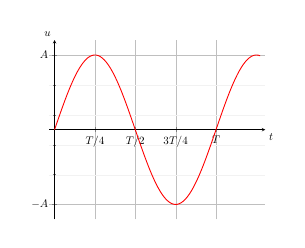
\begin{tikzpicture}[scale=0.4]
                \begin{axis}%
                    [grid=both,
                    minor tick num=4,
                    grid style={line width=.1pt, draw=gray!10},
                    major grid style={line width=.2pt,draw=gray!50},
                    axis lines=middle,
                    enlargelimits={abs=0.2},
                    xlabel={$t$},
                    ylabel={$u$},
                    xlabel style={below right},
                    ylabel style={above left},
                    xtick={pi/2,pi,3*pi/2, 2*pi},
                    xticklabels={$T/4$,$T/2$,$3T/4$,$T$},
                    ytick={-1,1},
                    yticklabels={$-A$,$A$}
                    ]
                    \addplot[domain=0:8,samples=100,smooth,red,thick] {cos(deg(x-pi/2))};
                \end{axis}
            \end{tikzpicture}
        \end{column}
    \end{columns}
\end{frame}

\begin{frame}{Problemas do Halliday, capítulo 15}
    \centering
    \includegraphics<+>[width=\textwidth]{images/Captura de tela de 2024-01-25 13-33-22.png}

    \includegraphics<+>[width=\textwidth]{images/Captura de tela de 2024-01-25 13-33-48.png}

    \includegraphics<+>[width=\textwidth]{images/Captura de tela de 2024-01-25 13-45-08.png}
\end{frame}

\begin{frame}{Fim do assunto para a 1\esima{} prova}
    Lista de exercícios:
    \begin{itemize}
        \item Problemas 3, 6, 16 e 35 do capítulo 12 do Halliday
        \item Problemas 1, 5, 6, 10, 12, 13, 14, 15, 31, 32, 33, 44, 45, 46 e 50 do capítulo 14 do Halliday
        \item Problemas 1, 2, 3, 5, 6, 7, 8, 12 e 20 do capítulo 15 do Halliday
    \end{itemize}

    A prova terá entre 3 e 4 problemas da lista com \textit{valores numéricos modificados}

\end{frame}

% \begin{frame}{Alteração no texto do problema 44 do capítulo 14 do Halliday}
%     Versão do livro:
%     \begin{center}
%         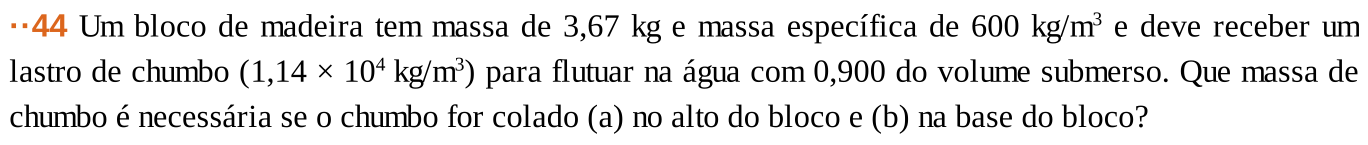
\includegraphics[width=\textwidth]{images/problema 44.png}
%     \end{center}

%     \begin{block}{Versão do professor}
%         Um bloco de madeira tem massa \SI{3.67}{kg} e massa específica de \(\SI{600}{kg/m^3}\)
%         e deve receber um lastro de chumbo (\(\SI{1.14e4}{kg/m^3}\)) para flutuar na água
%         com \num{0.900} do volume \textbf{do bloco de madeira} submerso. Que massa de chumbo é necessária
%         se o chumbo for colado (a) no alto do bloco e (b) na base do bloco?
%     \end{block}

% \end{frame}

\begin{frame}{Alguns sistemas que apresentam MHS}
    \begin{itemize}
        \begin{columns}[c]
            \begin{column}{0.45\textwidth}
                \item Um bloco/corpo de massa \(m\) preso a uma mola com constante de força \(k\)
                    \[
                        \omega=\sqrt{\frac{k}{m}}
                    \]
                \end{column}

                \begin{column}{0.45\textwidth}
                    \centering
                    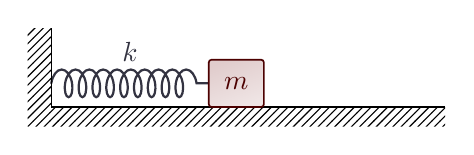
\begin{tikzpicture}[
                        ground/.style={fill,pattern=north east lines,draw=none,minimum width=0.3,minimum height=0.6},
                        spring/.style={line width=0.8,blue!7!black!80,decorate, decoration={coil,amplitude=5,segment length=5},line cap=round},
                        mass/.style={line width=0.6,red!30!black,fill=red!40!black!10,rounded corners=1,
                        top color=red!40!black!20,bottom color=red!40!black!10,shading angle=20}
                        ]
                        \def\H{1}    % wall height
                        \def\T{0.3}  % wall thickness
                        \def\W{5.0}  % ground length
                        \def\D{0.25} % ground depth
                        \def\h{0.6}  % mass height
                        \def\w{0.7}  % mass width
                        \def\x{1.6}  % mass x position

                        \foreach \y/\x in {0/2.0} {
                            \begin{scope}[shift={(0,-\y)}]
                                \draw[spring] (0,\h/2) --++ (\x,0) node [midway, above, yshift=1ex] {$k$};
                                \draw[ground] (0,0) |-++ (-\T,\H) |-++ (\T+\W,-\H-\D) -- (\W,0) -- cycle;
                                \draw (0,\H) -- (0,0) -- (\W,0);
                                \draw[mass] (\x,0) rectangle++ (\w,\h) node[midway] {$m$};
                            \end{scope}
                        }
                    \end{tikzpicture}
                \end{column}
            \end{columns}

            \vspace{\fill}

            \begin{columns}[T]
                \begin{column}{0.45\textwidth}
                \item Um pêndulo simples (\(\theta\) pequeno) com 
                    comprimento \(L\)
                    \[
                        \omega=\sqrt{\frac{g}{L}}
                    \]
                \end{column}

                \begin{column}{0.45\textwidth}
                    \centering
                    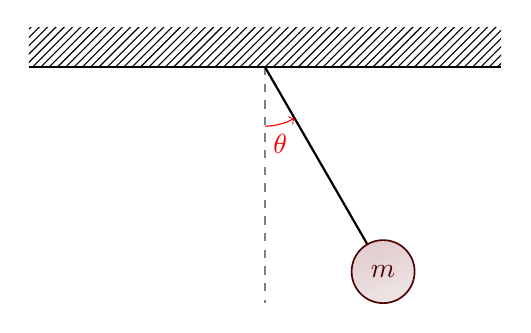
\begin{tikzpicture}[
                        mass/.style={line width=0.6,red!30!black,fill=red!40!black!10,rounded corners=1,
                        top color=red!40!black!20,bottom color=red!40!black!10,shading angle=20}
                        ]
                        \coordinate (origo) at (0,0);
                        \coordinate (pivot) at (1,5);
                        \draw[thick,gray,dashed] (origo) -- ++(0,-3) coordinate (mary);
                        % draw roof
                        \fill[pattern = north east lines] ($ (origo) + (-3,0) $) rectangle ($ (origo) + (3,0.5) $);
                        \draw[thick] ($ (origo) + (-3,0) $) -- ($ (origo) + (3,0) $);

                        \draw[thick] (origo) -- ++(300:3) coordinate (bob);
                        \draw [mass] (bob) node {$m$} circle (0.4);

                        \draw [red,->] ($(origo)+(0,-0.75)$) arc (270:300:0.75) node [midway,below] {$\theta$};
                \end{tikzpicture}
            \end{column}
        \end{columns}
    \end{itemize}
\end{frame}

\begin{frame}{Problemas do Halliday, capítulo 15}
    \centering
    \includegraphics<+>[width=\textwidth]{images/Captura de tela de 2024-02-06 09-50-26.png}

    % \includegraphics<+>[width=\textwidth]{images/problemas_91e82.png}
\end{frame}

\begin{frame}{Problemas do Tipler, capítulo 14}
    \centering
    \includegraphics<+>[width=\textwidth]{images/Captura de tela de 2023-12-19 11-37-44.png}
\end{frame}

\begin{frame}{Atividade}
    \begin{itemize}
        \item Vale 15\% da \(N_2\)
        \item Ler as seções 15-5 (\textit{Oscilações amortecidas}) e 15-6 
            (\textit{Oscilações forçadas e ressonância}) do capítulo 15 do Halliday, tirando
            dúvidas com o professor quando necessário
        \item Resolva e entregue os problemas 59 e 62 do capítulo 15 do Halliday
        \item Pode ser digitado ou manuscrito
        \item Grupo de no máximo 2 alunos\footnote{Pode ser feito individual}
        \item Data de entrega: \textit{a definir}
    \end{itemize}
\end{frame}

\begin{frame}
    \frametitle{Movimento ondulatório}
    \begin{itemize}
        \item Uma \textbf{onda} surge quando um sistema é deslocado de sua posição de
            equilíbrio e a perturbação se propaga de uma região para outra do
            sistema com \textit{velocidade definida} 
        \item Quando uma onda se propaga, ela carrega energia e momento linear, mas
            não há transporte de matéria
    \end{itemize}
    \centering
    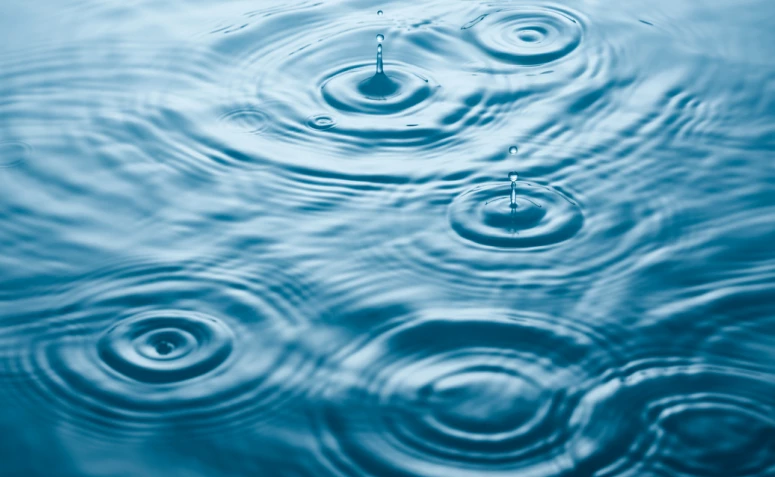
\includegraphics[height=\textheight-90pt]{images/ondas.png}
\end{frame}

\begin{frame}
    \begin{itemize}
        \item Quando os deslocamentos do meio são perpendiculares à direção de
            propagação, temos uma \textbf{onda transversal}
        \item Quando os deslocamentos do meio são paralelos à direção de
            propagação, temos uma \textbf{onda longitudinal}
            \vspace{\fill}
            \begin{columns}
                \begin{column}{0.4\textwidth}
                    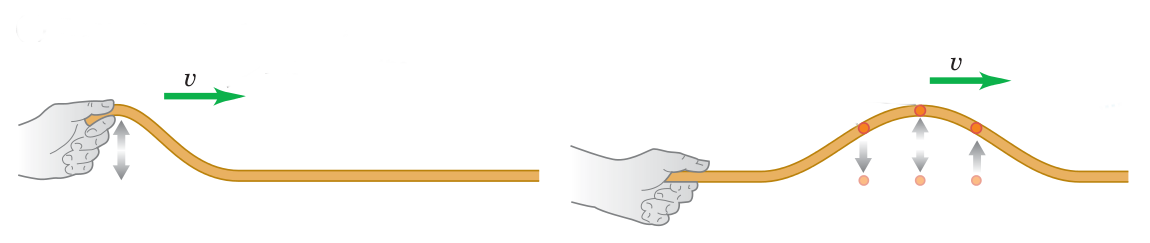
\includegraphics[width=\textwidth]{images/transversal.png}
                    \centering \textbf{transversal}
                \end{column}

                \begin{column}{0.4\textwidth}
                    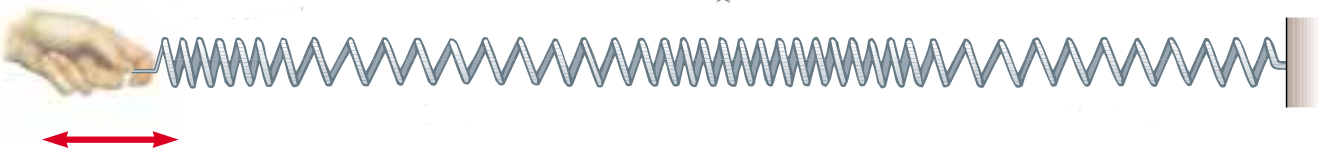
\includegraphics[width=\textwidth]{images/longitudinal.png}
                    \centering \textbf{longitudinal}
                \end{column}
            \end{columns}
        \item Quando a onda precisa de um meio para se propagar, temos uma \textbf{onda mecânica}
        \item O som é um exemplo de onda mecânica
        \item Quando não é necessário um meio de propagação, temos uma \textbf{onda eletromagnética}
        \item A luz é um exemplo de onda eletromagnética
    \end{itemize}
\end{frame}

\begin{frame}
    \frametitle{Função de onda}
    \begin{itemize}
        \item Considere que a posição $y$ em função do tempo de um ''pedaço'' de corda na posição $x$ é dada por 
            \[
                y(x,t)=\frac{2}{(x-3,0t)^2+1}
            \]
            com $y$ e $x$ em centímetros e $t$ em segundos. Os gráficos da
            função nos tempos $t=\SI{0.0}{s}$, $t=\SI{1.0}{s}$ e
            $t=\SI{2.0}{s}$ são dados a seguir
    \end{itemize}
    \centering
    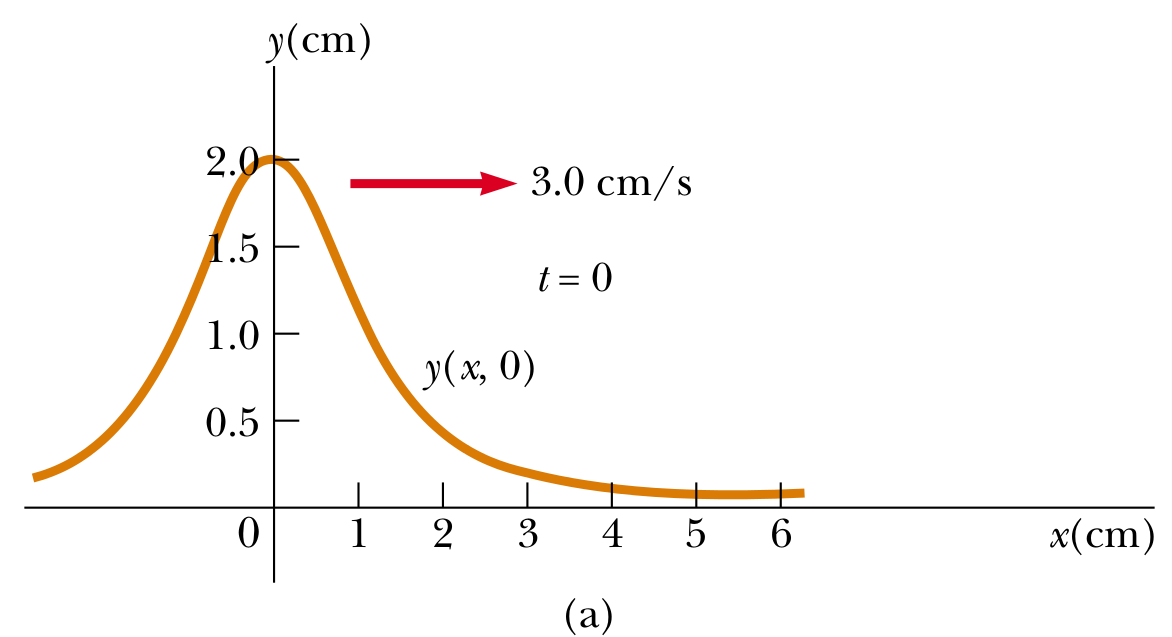
\includegraphics[width=0.32\textwidth]{images/t-0}
    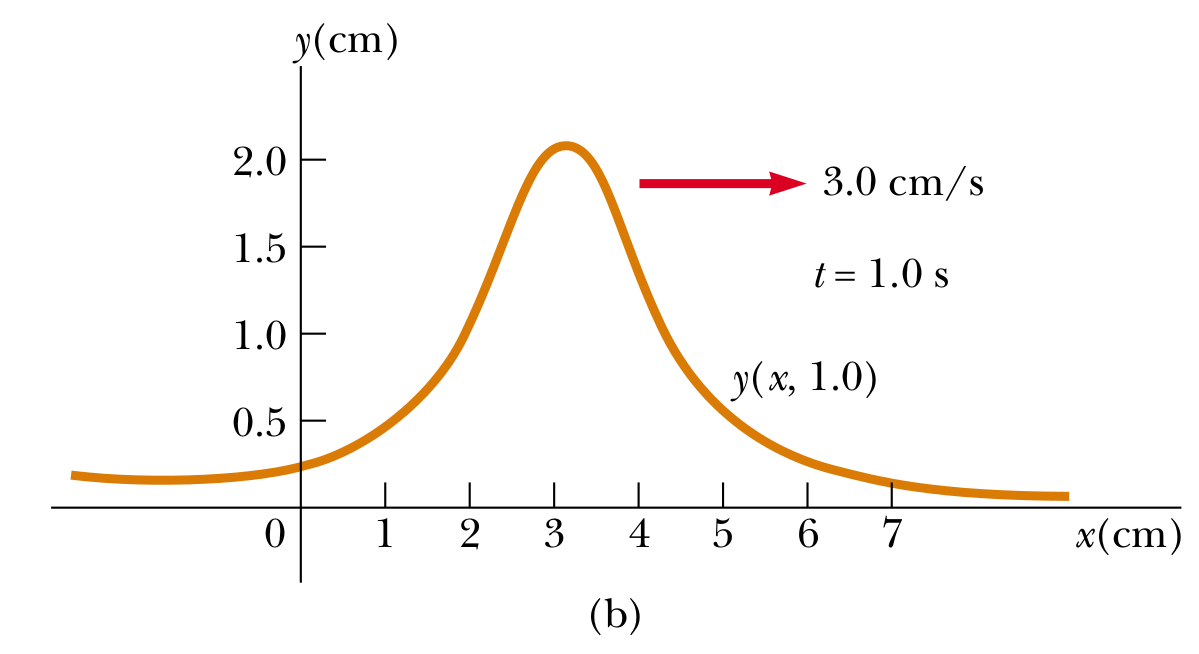
\includegraphics[width=0.32\textwidth]{images/t-1}
    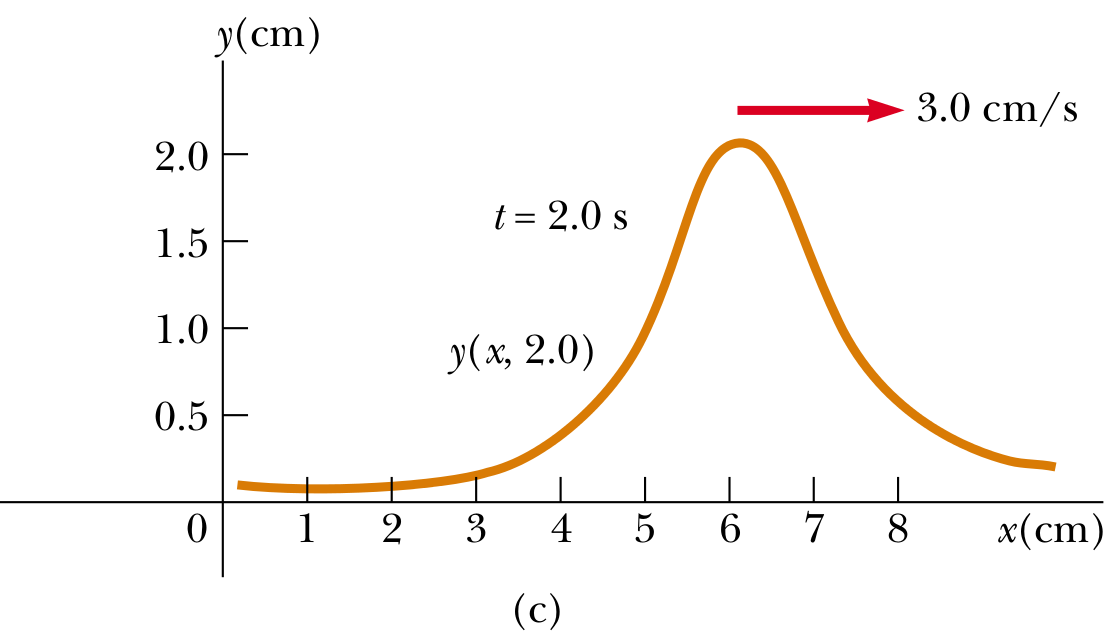
\includegraphics[width=0.32\textwidth]{images/t-2}
\end{frame}

\begin{frame}
    \begin{itemize}
        \item Observe que a ''forma'' da onda não se altera:
            \[
                y(x,0) = y(x',1)=y(x'',2)
            \]
            onde $x'=x-3$ e $x''=x-6$. De forma geral, podemos dizer que
            \[
                y(x,t)=y(x-3t)
            \]

        \item Dizemos que a função $y(x,t)$ é uma \textbf{função de onda}, uma
            representação matemática de uma onda
        \item Todas as funções de onda têm a forma
            \begin{align*}
                y(x,t)=f(x-vt) & ~~\rightarrow~~ \text{onda movendo-se no sentido +x}\\
                y(x,t)=f(x+vt) & ~~\rightarrow~~ \text{onda movendo-se no sentido -x}
            \end{align*} 
    \end{itemize}
\end{frame}

\begin{frame}
    \frametitle{Equação da onda}
    Todas as funções de onda são soluções da equação diferencial da onda:
    \[
        \frac{\partial^2 y}{\partial x^2} = \frac{1}{v^2}\frac{\partial^2 y}{\partial t^2}
    \]

    Ou seja: da mesma forma que fizemos com o MHS, uma onda é um sistema cuja
    representação matemática (função de onda) é solução da equação da onda

    \vfill

    \pause
    Mostre que \(y(x,t)=f(x\mp vt)\) é solução da equação da onda
\end{frame}

\begin{frame}{Ondas harmônicas}
    \begin{itemize}
        \item Ondas harmônicas são o tipo mais básico de ondas periódicas
        \item  Todas as ondas, periódicas ou não, podem ser modeladas como 
            uma superposição de ondas harmônicas\footnote{Quem quiser mais 
            detalhes basta procurar por \textit{Série de Fourier}}
        \item A função de onda de uma onda harmônica\footnote{...propagando
            ao longo do eixo \(x\), no sentido positivo...} é dada por
            \[
                y(x,t)=A\sen{(kx-\omega t+\delta)}
            \]
            onde
            \begin{description}
                \item[k] é o número de onda
                \item[$\omega$] é a frequência angular
                \item[$\delta$] é a constante de fase
            \end{description}
        \item \textit{Podemos demonstrar que}
            \[
                v=\frac{\omega}{k}
            \]
    \end{itemize}
\end{frame}

\begin{frame}{Período}
    Cada ''ponto'' em uma dada posição \(x\) de uma 
    onda harmônica executa um MHS com um período \(T\) e 
    frequência \(f\), onde
    \[
        y(x,t_n) = y(x,t_n+T), \qquad T=\frac{1}{f}, \qquad \omega=2\pi f = \frac{2\pi}{T}
    \]

    \vspace{\fill}\centering
    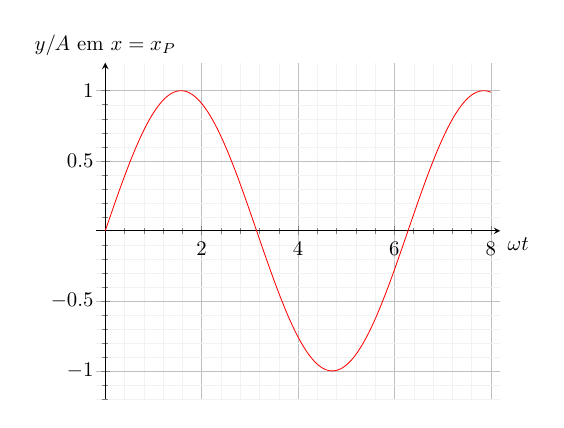
\begin{tikzpicture}[scale=0.75]
        \begin{axis}%
            [
            grid=both,
            minor tick num=4,
            grid style={line width=.1pt, draw=gray!10},
            major grid style={line width=.2pt,draw=gray!50},
            axis lines=middle,
            enlargelimits={abs=0.2},
            xlabel={$\omega t$},
            ylabel={$y/A$ em $x=x_P$},
            xlabel style={below right},
            ylabel style={above},
            ]
            \addplot[domain=0:8,samples=200,smooth,red] {sin(deg(x))};
        \end{axis}
    \end{tikzpicture}
\end{frame}

\begin{frame}{Comprimento de onda}
    Em um tempo \(t_n\), a ''forma'' de uma onda se repete em intervalos
    de posição iguais ao \textit{comprimento de onda} \(\lambda\), ou seja
    \[
        y(x_P,t) = y(x_P+\lambda,t), \qquad k=\frac{2\pi}{\lambda}
    \]

    \vspace{\fill}\centering
    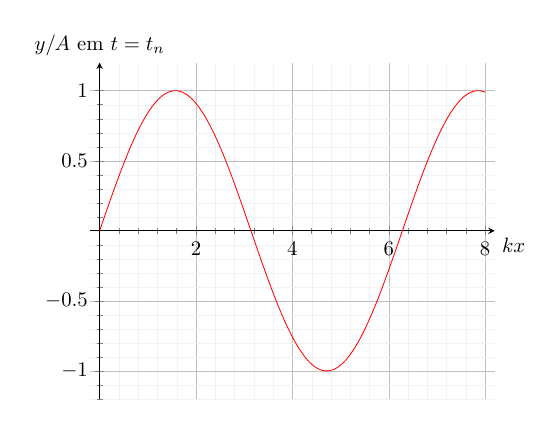
\begin{tikzpicture}[scale=0.75]
        \begin{axis}%
            [
            grid=both,
            minor tick num=4,
            grid style={line width=.1pt, draw=gray!10},
            major grid style={line width=.2pt,draw=gray!50},
            axis lines=middle,
            enlargelimits={abs=0.2},
            xlabel={$kx$},
            ylabel={$y/A$ em $t=t_n$},
            xlabel style={below right},
            ylabel style={above},
            ]
            \addplot[domain=0:8,samples=200,smooth,red] {sin(deg(x))};
        \end{axis}
    \end{tikzpicture}
\end{frame}

% \begin{frame}{Exercício de revisão}
%     \begin{itemize}
%         \item Uma onda harmônica tem função de onda
%             \[
%                 y(x,t) = A \sen{(kx-\omega t+\delta)}
%             \]
%             onde \(A=\SI{3}{cm}\), \(k=\SI{2.2}{m^{-1}}\), \(\omega = \SI{3.5}{s^{-1}}\)
%             e \(\delta=\pi/2\)
%         \item Temos que \(y(x_P,0)=A/4\) e \(y\) \textit{está diminuindo com o tempo}
%         \item Determine o menor valor de \(\lvert x_Q-x_P\rvert\), onde \(y(x_Q,0)=0\) e
%             \begin{itemize}
%                 \item \(x_Q > x_P\)
%                 \item \(x_Q < x_P\)
%             \end{itemize}
%     \end{itemize}
% \end{frame}

% \begin{frame}
%     \begin{tikzpicture}[scale=0.85]
%         \begin{axis}%
%             [
%             grid=both,
%             minor tick num=4,
%             grid style={line width=.1pt, draw=gray!10},
%             major grid style={line width=.2pt,draw=gray!50},
%             axis lines=middle,
%             enlargelimits={abs=0.2},
%             xlabel={$kx$},
%             ylabel={$y/A$ em $t=0$},
%             xlabel style={below right},
%             ylabel style={above},
%             ]
%             \addplot[domain=-8:8,samples=200,smooth,red] {sin(deg(x)+90)};
%         \end{axis}
%     \end{tikzpicture}%
%     \hspace{\fill}%
%     \begin{tikzpicture}[scale=0.85]
%         \begin{axis}%
%             [
%             grid=both,
%             minor tick num=4,
%             grid style={line width=.1pt, draw=gray!10},
%             major grid style={line width=.2pt,draw=gray!50},
%             axis lines=middle,
%             enlargelimits={abs=0.2},
%             xlabel={$\omega t$},
%             ylabel={$y/A$ em \color{red}$x=0$},
%             xlabel style={below right},
%             ylabel style={above},
%             ]
%             \addplot[domain=-8:8,samples=200,smooth,red] {sin(deg(x)+90)};
%         \end{axis}
%     \end{tikzpicture}

%     \centering
%     \includegraphics<2->[height=\textheight-180pt]{../fis4/images/Captura de tela de 2023-12-14 19-04-21.png}
% \end{frame}

% \begin{frame}{Atividade}
%     \begin{itemize}
%         \item Vale 12\% da \(N_2\)
%         \item Fazer uma pesquisa sobre \textit{Efeito Doppler} e resolver 2 
%             problemas relacionados a ele
%         \item Pode ser digitado ou manuscrito
%         \item Grupo de no máximo 2 alunos\footnote{Pode ser feito individual}
%         \item Entrega até o dia 29/2 na Sala de Aula
%     \end{itemize}
% \end{frame}

% \begin{frame}{Atividade}
%     \begin{itemize}
%         \item Vale 15\% da \(N_2\)
%         \item Fazer uma pesquisa sobre \textit{Ondas estacionárias e ressonância} (Seção 16-7 do livro)
%         \item Não é para copiar o texto do livro: pesquise em outras fontes e \textbf{resuma}
%         \item Pode ser digitado ou manuscrito
%         \item Grupo de no máximo 2 alunos\footnote{Pode ser feito individual}
%         \item Enviar até 14/03 para o Sala de Aula
%     \end{itemize}
% \end{frame}

\begin{frame}{Exercícios do Halliday, capítulo 16}
    \includegraphics<+>[width=\textwidth]{images/Captura de tela de 2024-02-08 14-36-09.png}

    \includegraphics<+>[width=\textwidth]{images/Captura de tela de 2024-02-08 14-40-57.png}

    \includegraphics<+>[width=\textwidth]{images/Captura de tela de 2024-02-08 14-42-03.png}


\end{frame}

\begin{frame}
    \begin{block}{Exercício do Halliday, capítulo 16}
        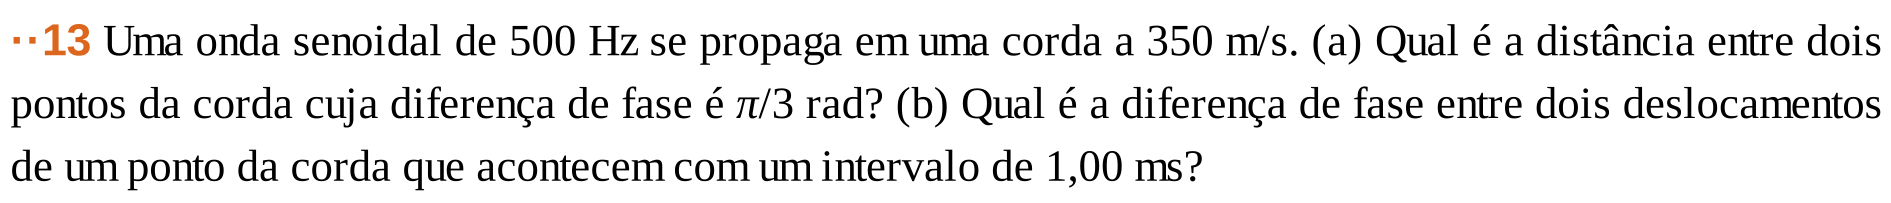
\includegraphics[width=\textwidth]{images/Captura de tela de 2024-06-18 08-41-37.png}
    \end{block}

    \begin{block}{Exercício do Tipler, capítulo 15}
        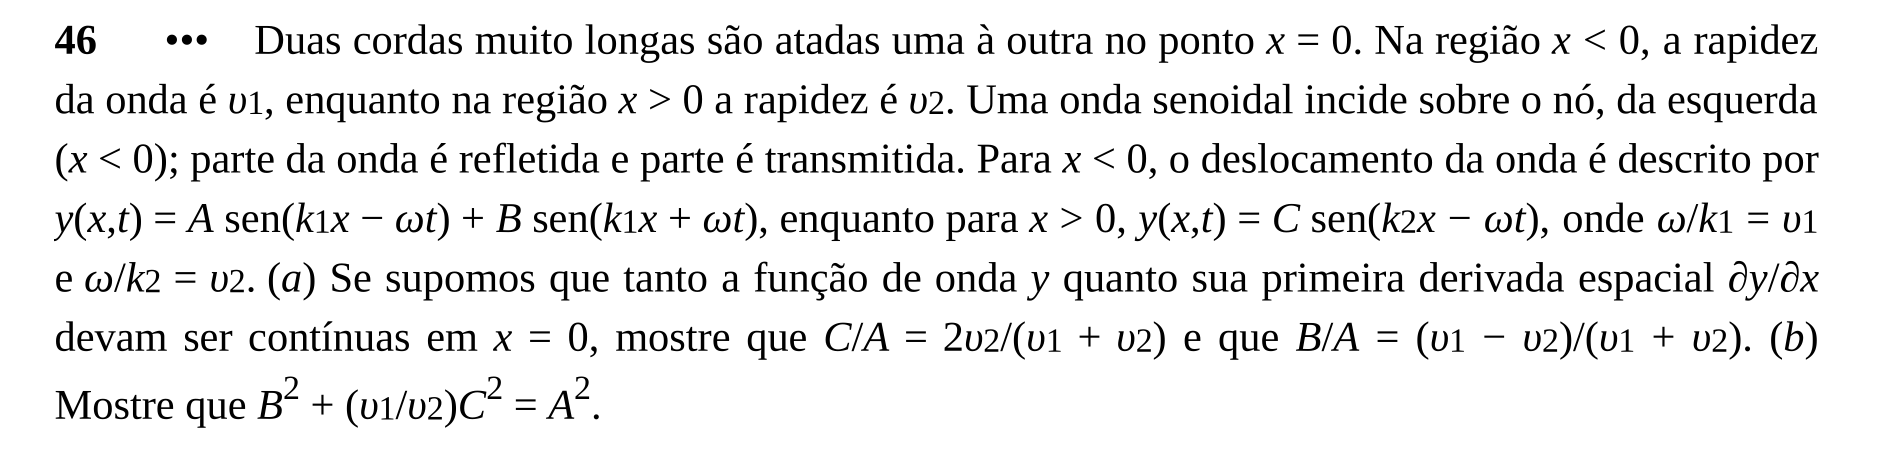
\includegraphics[width=\textwidth]{images/Captura de tela de 2024-06-18 08-57-22.png}
    \end{block}
\end{frame}

\begin{frame}[c]
    \frametitle{Superposição de ondas}

    \begin{block}{Princípio da superposição}
        Se duas ou mais ondas se propagam por um meio, o valor resultante da função de onda em qualquer ponto é a soma algébrica dos valores
        das funções de onda das ondas individuais
    \end{block}
\end{frame}

\begin{frame}
    \frametitle{Interferência}

    \begin{itemize}
        \item Sejam duas ondas harmônicas que diferem apenas na fase incidindo em um ponto
            \[
                y=y_1 + y_2 = A \left[ \sen{(kx -\omega t + \delta)} + \sen{(kx -\omega t)} \right]
            \]
        \item Mas 
            \[
                \sen{\theta_1} + \sen{\theta_2} = 
                2\cos{\left[\frac{\theta_1 - \theta_2}{2}\right]}
                \sen{\left[\frac{\theta_1 + \theta_2}{2}\right]}
            \]
        \item Assim
            \[
                y=2A
                \cos{\left(\frac{\delta}{2}\right)}
                \sen{\left(kx -\omega t + \frac{\delta}{2}\right)}
            \]
            ou seja, a amplitude da onda resultante depende da diferença de fase \(\delta\)
    \end{itemize}
\end{frame}

\begin{frame}
    Se \(\delta=2m\pi\), onde \(m=0, 1, 2,\ldots\) temos que 
    \[
        \cos{\left(\frac{\delta}{2}\right)} = \cos{\left(\frac{2m\pi}{2}\right)} = \pm 1
        \qquad (\text{lembre-se que } \sen{(\theta + \pi)} = -\sen\theta)
    \]
    ou seja, a amplitude da onda resultante é o dobro da amplitude das ondas incidentes. Nesse caso, temos uma \textbf{interferência construtiva}

    %http://tex.stackexchange.com/a/162650
    \begin{center}
        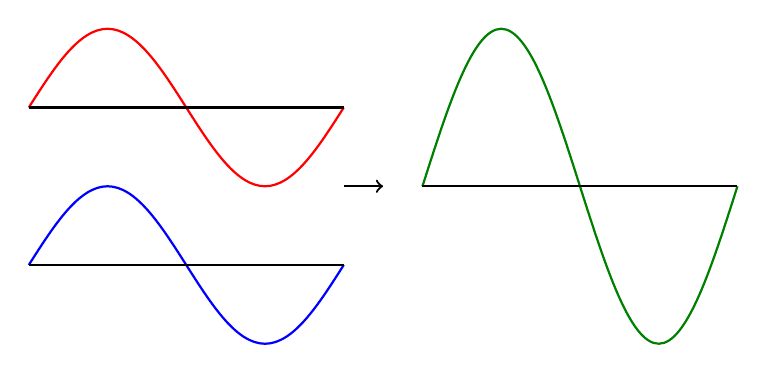
\begin{tikzpicture}
            \draw[thick,red] (0,0) sin (1,1) cos (2,0) sin (3,-1) cos (4,0);
            \draw[thick,blue] (0,-2) sin (1,-1) cos (2,-2) sin (3,-3) cos (4,-2);
            \draw[thick,->] (4,-1) -- (4.5,-1);
            \draw[thick,green!50!black] (5,-1) sin (6,1) cos (7,-1) sin (8,-3) cos (9,-1);
            \draw [thick] (0,0) -- (4,0);
            \draw [thick] (0,-2) -- (4,-2);
            \draw [thick] (5,-1) -- (9,-1);
        \end{tikzpicture}
    \end{center}
\end{frame}

\begin{frame}
    Se \(\delta=(2m+1)\pi\), onde \(m=0, 1, 2,\ldots\) temos que 
    \[
        \cos{\left(\frac{\delta}{2}\right)} = \cos{\left(\frac{(2m+1)\pi}{2}\right)} = 0
    \]
    ou seja, a amplitude da onda resultante é zero. Nesse caso, temos uma \textbf{interferência destrutiva}

    %http://tex.stackexchange.com/a/162650
    \begin{center}
        \begin{tikzpicture}
            \draw[thick,red] (0,0) sin (1,1) cos (2,0) sin (3,-1) cos (4,0);
            \draw[thick,blue] (0,-2.5) sin (1,-3.5) cos (2,-2.5) sin (3,-1.5) cos (4,-2.5);
            \draw[thick,->] (4,-1.25) -- (4.5,-1.25);
            \draw[thick] (0,0) -- (4,0);
            \draw[thick] (0,-2.5) -- (4,-2.5);
            \draw[thick] (5,-1.25) -- (9,-1.25);
        \end{tikzpicture}
    \end{center}
\end{frame}

\begin{frame}
    \frametitle{Diferença de fase devido à diferença de percurso}
    \begin{itemize}
        \item Sejam duas ondas harmônicas iguais em um ponto inicial
            (\(x=0\)), mas que percorrem \textit{diferentes caminhos} para chegar em um
            ponto final durante \textit{o mesmo intervalo de tempo}
            \begin{center}
                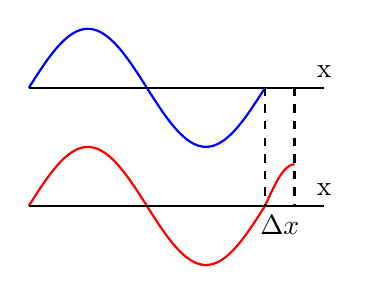
\begin{tikzpicture}[scale=0.75]
                    \draw[thick,blue] (0,0) sin (1,1) cos (2,0) sin (3,-1) cos (4,0);
                    \draw[thick,red] (0,-2) sin (1,-1) cos (2,-2) sin (3,-3) cos (4,-2) sin (4.5, -1.2929);
                    \draw [thick] (0,0) -- (5,0) node [anchor = south] {x};
                    \draw [thick] (0,-2) -- (5,-2) node [anchor = south] {x};
                    \draw [thick, dashed] (4,0) -- (4,-2);
                    \draw [thick, dashed] (4.5,0) -- (4.5,-2);
                    \draw (4.25,-2) node [anchor = north] {\(\Delta x\)};
                \end{tikzpicture}
            \end{center}
        \item No ponto final, temos que
            \begin{align*}
                y_1 &= A \sen{(kx -\omega t)} \\
                y_2 &= A \sen{(k(x+\Delta x) -\omega t)} = A \sen{(kx -\omega t +k\Delta x)}
            \end{align*}
            ou seja: \(\delta = k\Delta x = \dfrac{2\pi\Delta x}{\lambda}\)
    \end{itemize}
\end{frame}

\begin{frame}
    \begin{itemize}
        \item Temos interferência construtiva quando \(\delta=2m\pi\) de forma que
            \[
                \frac{2\pi\Delta x}{\lambda} = 2m\pi \qquad \rightarrow \qquad \Delta x = m\lambda
            \]
        \item Temos interferência destrutiva quando \(\delta=(2m+1)\pi\) de forma que
            \[
                \frac{2\pi\Delta x}{\lambda} = (2m+1)\pi \qquad \rightarrow \qquad \Delta x = (2m+1)\frac{\lambda}{2}
            \]
    \end{itemize}
    onde, em ambos os casos, \(m=0,1,2\ldots\)
\end{frame}

\begin{frame}{Exercícios do Tipler, capítulo 16}
    \centering
    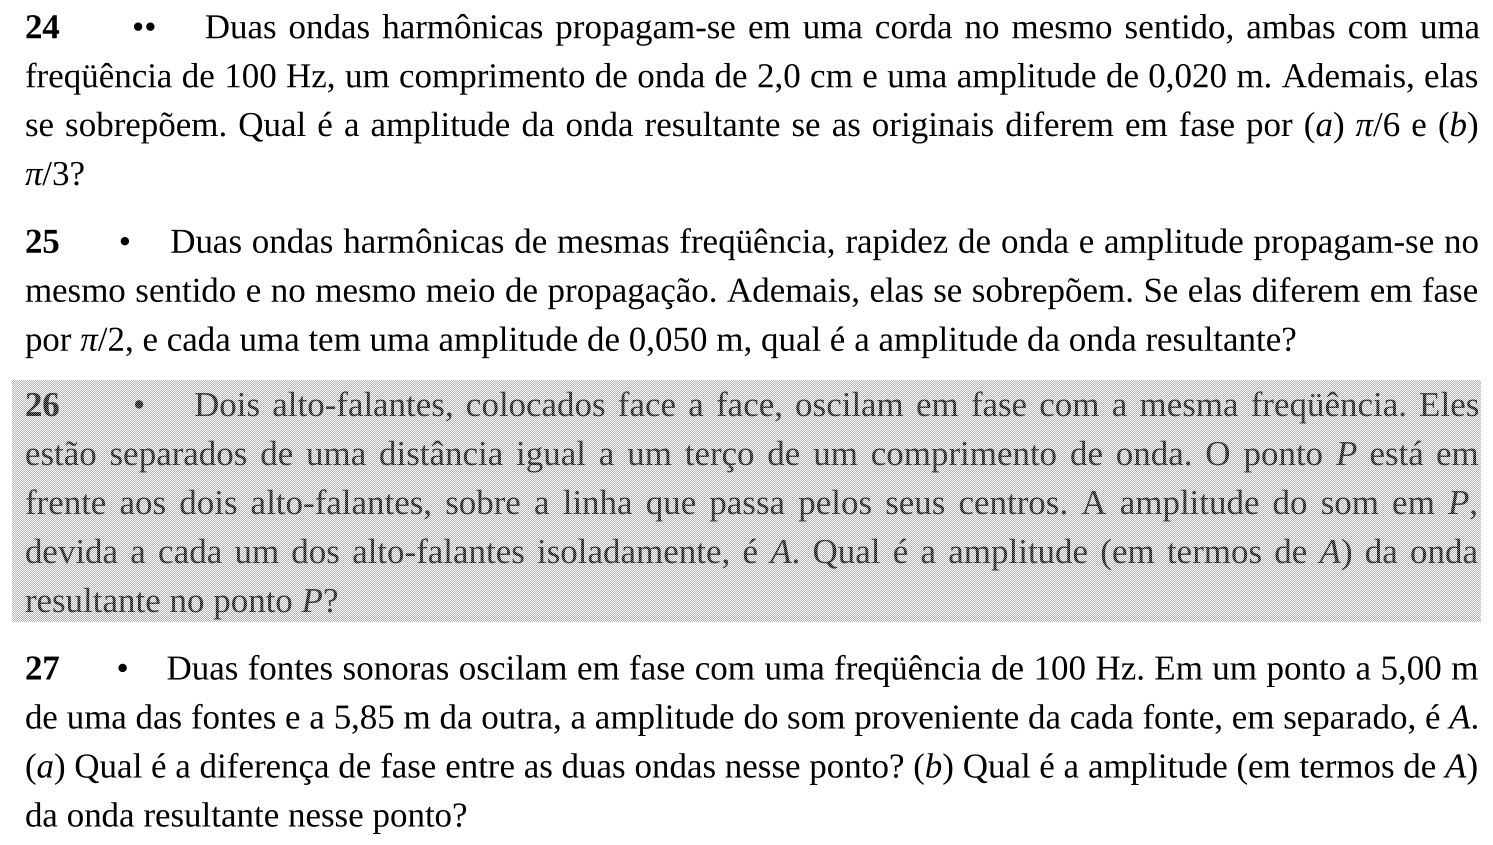
\includegraphics[height=\textheight-28pt]{images/Captura de tela de 2024-01-30 10-31-40.png}
\end{frame}

\begin{frame}{Atividade}
    \begin{itemize}
        \item Vale 15\% da \(N_2\)
        \item Grupo de no máximo 3 alunos
        \item Faça uma pesquisa sobre \textit{Ondas sonoras} que responda as seguintes questões
            \begin{enumerate}
                \item  Qual é a fórmula para a velocidade do som? De que propriedades do meio de propagação ela depende?
                \item  Qual é a velocidade do som no ar? 
                \item  Qual a dependência da velocidade do som no ar com a temperatura?
                \item  Fale sobre a escala decibel de intensidade sonora
                \item  Fale sobre o efeito Doppler
            \end{enumerate}
        \item \alert{Não é para fazer no formato \textit{questão+resposta}: é um texto
            que fale sobre ondas sonoras e responda as questões}
    \end{itemize}
\end{frame}


\section{Termodinâmica}

\begin{frame}{Temperatura} 
    \begin{itemize} 
        \item Associamos o conceito de temperatura a quão quente ou frio um corpo está quando nele
            tocamos, mas essa avaliação não é confiável nem quantitativa 
        \item Dizemos que dois ou mais corpos estão em \textbf{contato térmico} quando
            pode haver troca de \textbf{energia} entre eles devido à diferença de
            temperatura 
        \item Dizemos que dois ou mais corpos estão em
            \textbf{equilíbrio térmico} se quando forem colocados em contato térmico
            não houver troca de \textbf{energia} devido à diferença de temperatura, ou
            seja, estão na mesma temperatura 
            \begin{block}{Lei zero da Termodinâmica} 
                Se dois corpos estão em equilíbrio térmico com um terceiro,
                então os três corpos estão em equilíbrio térmico entre si 
            \end{block} \pause
        \item Assim, podemos pensar na temperatura como a propriedade que determina se
            um corpo está em equilíbrio térmico com outro 
    \end{itemize} 
\end{frame}
%
\begin{frame}
    \begin{itemize}
        \item Uma propriedade física que varia com a temperatura é chamada de
            \textbf{propriedade termométrica}
        \item Usando a lei zero e um corpo com uma propriedade termométrica
            mensurável, podemos construir um \textbf{termômetro}
        \item Colocamos o termômetro em contato térmico com um corpo A e
            medimos a propriedade termométrica no equilíbrio térmico
        \item Colocamos o termômetro em contato térmico com um corpo B e
            medimos a propriedade termométrica no equilíbrio térmico
        \item Se o valor medido para propriedade termométrica for igual para
            ambos os corpos, eles têm a mesma temperatura
        \item Além disso, podemos dar um valor para a temperatura a partir do
            valor medido da propriedade termométrica: podemos definir uma
            \textbf{escala termométrica}
    \end{itemize}
\end{frame}
%
\begin{frame}
    \frametitle{Algumas escalas}
    \begin{itemize}
        \item A \textbf{escala de temperatura centigrada ou Celsius} define a
            temperatura do ponto de gelo como sendo \SI{0}{\celsius} e a
            temperatura do ponto de vapor como sendo \SI{100}{\celsius}
        \item A \textbf{escala de temperatura Fahrenheit} define a temperatura
            do ponto de gelo como sendo \SI{32}{\degree F} e a temperatura do
            ponto de vapor como sendo \SI{212}{\degree F}
    \end{itemize}
    \pause
    \begin{block}
        {A escala de temperatura absoluta ou  escala Kelvin}

        \begin{itemize}
            \item Um gás ideal é definido como um gás onde a pressão, o volume e a temperatura se relacionam pela expressão
                \[
                    PV=nR(T-T_0)
                \]
                onde R=\SI{8.314}{J/(mol\ K)}, \(n\) é o número de moles do gás e \(T_0\) é a temperatura onde \(P=0\)

            \item A temperatura de \SI{0}{K} \textit{é definida como sendo} \(T_0\). Para efeito de comparação,
                \(T_0 = \SI{-273.15}{\celsius}\)

            \item A temperatura do \textbf{ponto triplo} da água é (\SI{273.16}{K}). Para efeito de comparação,
                o ponto triplo da água ocorre em \(T=\SI{0.01}{\celsius}\)
        \end{itemize}
    \end{block}
\end{frame}

\begin{frame}{Exercícios do \textbf{Tipler}, capítulo 17}
    \centering

    % \includegraphics<+>[height=\textheight-42pt]{images/tipler.png}

    \includegraphics<+>[width=\textwidth-37pt*\real{1.72}]{images/Captura de tela de 2024-02-20 10-14-55.png}

    \includegraphics<+>[width=\textwidth]{images/Captura de tela de 2024-02-20 10-23-50.png}

    % \includegraphics<+>[width=\textwidth-2pt*\real{1.77}]{../complementos/images/Captura de tela de 2024-02-20 10-22-11.png}
\end{frame}

% \begin{frame}{Lista de exercícios para a prova 2}
%     \begin{itemize}
%         \item Problemas 7, 8, 9 e 13 do capítulo 16 do Halliday
%         \item Problemas 24, 25 e 27 capítulo 16 do \textbf{Tipler}
%         \item Problemas  33, 34, 35, 36, 37, 41, 42, 43 e 44 do capítulo 17 do \textbf{Tipler}
%         \item A prova terá entre 3 e 4 problemas da lista com \textit{valores
%             numéricos modificados}
%     \end{itemize}
% \end{frame}

% \begin{frame}[c]
%     \centering
%     Fim do assunto para a segunda prova
% \end{frame}
\begin{frame}{Fim do assunto para a 2\esima{} prova}
    Lista de exercícios:
    \begin{itemize}
        \item Problemas 13 e 14 do capítulo 15 do Halliday
        \item Problemas 7, 8, 9 e 13 do capítulo 16 do Halliday
        \item Problemas 59, 60, 61, 62 e 63 do capítulo 14 do Tipler
        \item Problemas 46 do capítulo 15 do Tipler
        \item Problemas 24, 25 e 27 do capítulo 16 do Tipler
        \item Problemas 33, 34, 35, 36, 37, 41, 42, 43 e 44 do capítulo 17 do Tipler
    \end{itemize}
\end{frame}

\begin{frame}
    \frametitle{Calor e energia interna}
    \begin{itemize}
        \item \textbf{Energia interna} é toda a energia de um sistema associada
            a seus componentes microscópicos -- átomos e moléculas --
            \textit{quando vistos em um sistema de referência em repouso com
            relação ao centro de massa do sistema}. Essa última parte exclui a
            energia associada a fatores externos ao sistema, por exemplo, a
            energia cinética devido a movimentação pelo espaço

        \item \textbf{Calor} é definido como a transferência de energia através
            do limite de um sistema \textit{devido a uma diferença de
            temperatura} entre o sistema e sua vizinhança

            \begin{itemize}
                \item Calor \textbf{não é} a energia em uma substância quente
                \item Calor \textbf{não é} a ''quentura'' de uma substância
            \end{itemize}
    \end{itemize}
\end{frame}


\begin{frame}
    \frametitle{1\textordfeminine{} Lei -- conceitos básicos}
    \begin{itemize}
        \item Podemos aumentar a temperatura (e com isso a energia interna) de
            um sistema realizando \textbf{trabalho} sobre ele
        \item Na figura abaixo está um diagrama do aparato que Joule usou para
            determinar o trabalho necessário para aumentar a temperatura de uma
            quilo de água em \SI{1}{\celsius}
    \end{itemize}
    \begin{center}
        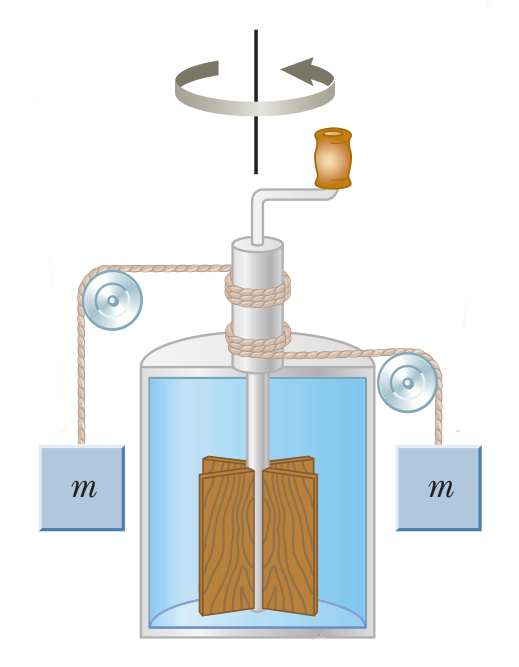
\includegraphics[width=0.3\textwidth-16pt*\real{0.78}]{images/joule.png}
    \end{center}
\end{frame}

\begin{frame}
    \frametitle{Interpretação molecular de calor e trabalho}
    \begin{center}
        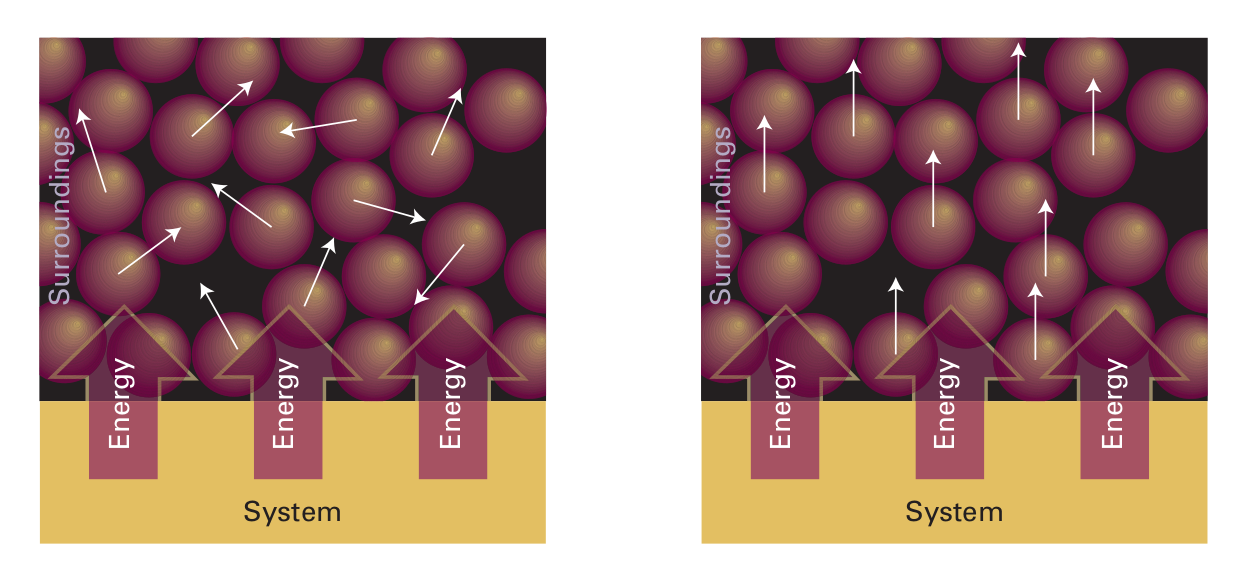
\includegraphics[width=0.75\textwidth]{images/trabalho_calor.png}
    \end{center}

    \begin{itemize}

        \item Quando energia é transferida na forma de calor, o movimento
            aleatório das moléculas da vizinhança do sistema é ''alterado''
        \item Quando energia é transferida na forma de trabalho, o movimento
            das moléculas da vizinhança do sistema é ''alterado'' de forma
            ordenada

    \end{itemize}
\end{frame}

\begin{frame}[c]
    \begin{block}{Primeira Lei da Termodinâmica}
        \begin{itemize}
            \item A variação da energia interna de um sistema é igual ao calor
                transferido para o sistema mais o trabalho realizado
                \textbf{sobre} o sistema
                \[
                    \Delta E_{\text{interna}} = Q_{\text{entra}} + W_{\text{sobre}}
                \]
            \item Outra forma de escrever a mesma coisa
                \[
                    \Delta E_{\text{interna}} = Q_{\text{entra}} - W_{\text{pelo}}
                \]
        \end{itemize}
    \end{block}
\end{frame}

\begin{frame}
    \frametitle{Capacidade térmica e calor específico}
    A quantidade de energia Q necessária para aumentar em \SI{1}{\celsius} a
    temperatura de uma \textbf{amostra} de uma substância é chamada de
    capacidade térmica da amostra
    \[
        C=\frac{Q}{\Delta T}
    \]

    O calor específico de uma substância é dada por
    \[
        c=\frac{C}{m}
    \]
    onde $m$ é a massa de uma amostra da substância que possui capacidade térmica $C$
\end{frame}

\begin{frame}
    A unidade de medida SI do calor é a mesma da energia, o joule.
    \begin{itemize}
        \item A caloria (cal) é definida como a quantidade de energia
            transferida necessária para elevar a temperatura de \SI{1}{g} de
            água de \SI{14.5}{\celsius} para \SI{15,5}{\celsius}
            \[
                \SI{1}{cal} = \SI{4,186}{J}
            \]
            Quando usado para descrever o valor energético de alimentos, muitas
            vezes o termo caloria se refere a quilocaloria

        \item A unidade térmica britânica (Btu) é definida como a quantidade de
            energia transferida necessária para elevar a temperatura de
            \SI{1}{libra} (\SI{4,448}{N}) de água de \SI{63}{\degree F} para
            \SI{64}{\degree F}
            \[
                \SI{1}{Btu} = \SI{252}{cal} = \SI{1054}{J}
            \]
    \end{itemize} 
\end{frame}

\begin{frame}[c]
    \frametitle{Calor específico da água}
    A definição original da caloria implica que o calor específico da água no estado líquido é
    \[
        c_{\text{água}} = \SI{1}{cal/g \celsius} = \SI{1}{kcal/kg  K} = 
        \SI{4,184}{kJ/kg K}
    \]

    Nos EUA, temos que
    \[
        c_{\text{água}} = \SI{1}{Btu/lb\degree F}
    \]

    O calor específico da água é muito maior do que o de outras substâncias
    comuns e por causa disso é um excelente material para armazenamento de
    energia térmica
\end{frame}

\begin{frame}{Exercícios do Halliday, capítulo 18}
    \centering
    \vboxcorr{50pt}{
        \begin{tikzpicture}
            \node [inner sep=0] (A) {
                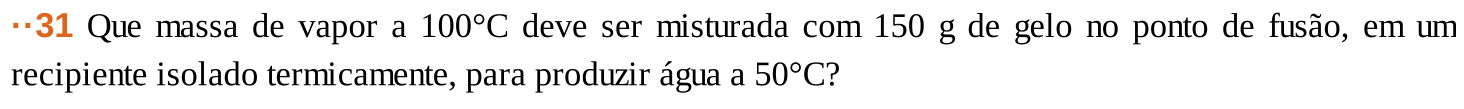
\includegraphics[width=\textwidth]{images/Captura de tela de 2025-05-28 12-03-18.png}
            };
            \node [inner sep=0, anchor=north west] at (A.south west) {
                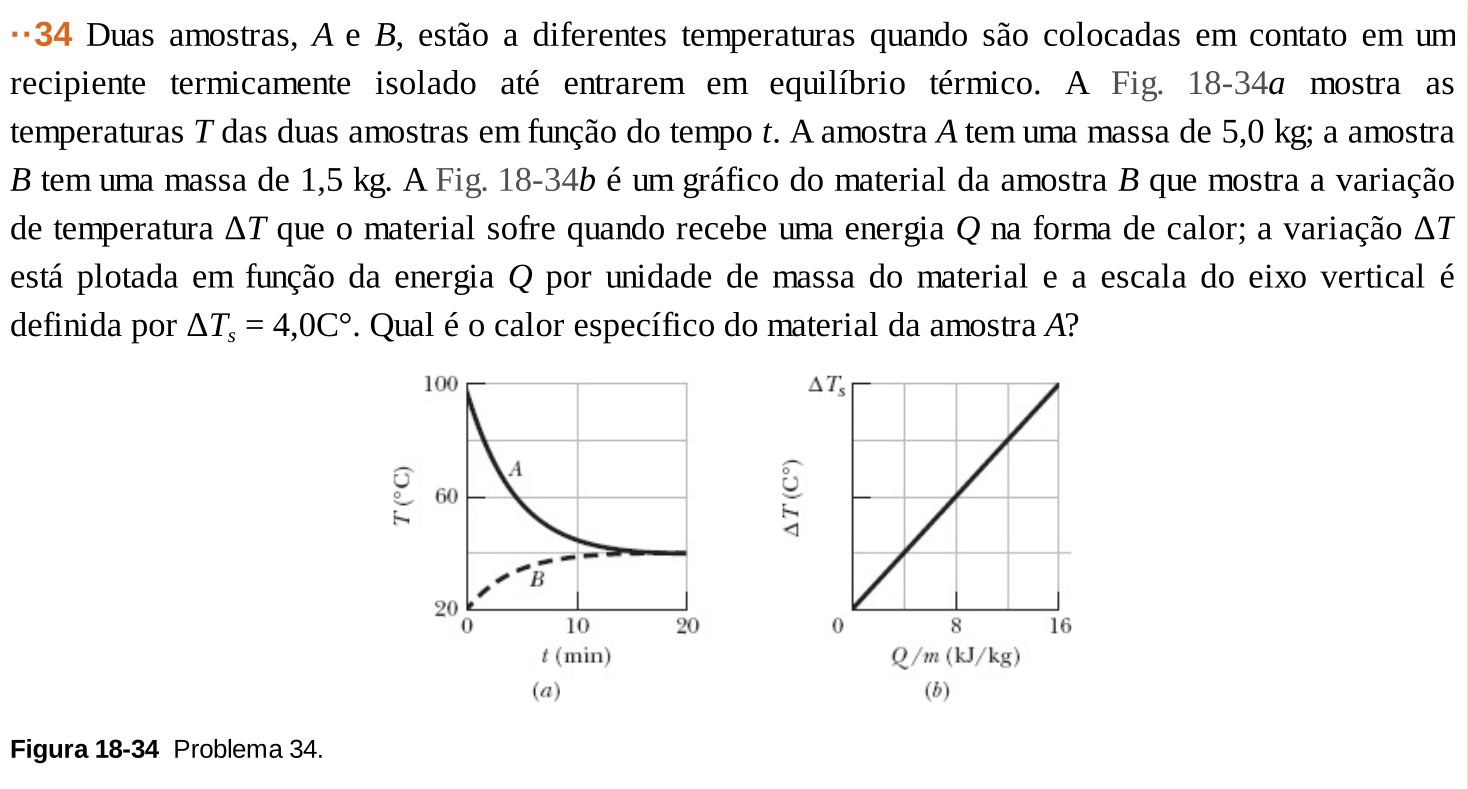
\includegraphics[width=\textwidth]{images/Captura de tela de 2025-05-28 12-07-45.png}
            };
        \end{tikzpicture}
        }
\end{frame}


\begin{frame}
    \frametitle{Trabalho realizado sobre um gás ideal por uma pressão constante}
    Seja um gás ideal confinado em um cilindro com um pistão bem ajustado e sem atrito
    \begin{center}
        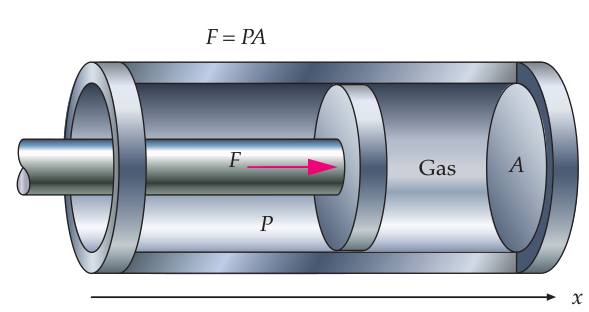
\includegraphics[width=0.425\textwidth]{images/quasistatic}
    \end{center}
    \begin{itemize}
        \item Quando o pistão se move uma pequena distância $\Delta x$, o
            trabalho realizado \textit{sobre o gás pelo pistão} é
            \[
                W_{\text{sobre~o~gás}} = F_x \Delta x=PA \Delta x=-P\Delta V
            \]
        \item Observe que para uma compressão $\Delta x > 0$ mas $\Delta V <
            0$, enquanto que para uma expansão ocorre o contrário
    \end{itemize}

\end{frame}

\begin{frame}[c]
    Se a pressão não é constante para todos os valores de \(x\), temos que
    \[
        W_{\text{sobre~o~gás}} = \lim_{\Delta V \to 0}  \sum (-P\Delta V) = -\int\limits_{V_i}^{V_f} PdV
    \]
    \pause
    Além disso,
    \[
        W_{\text{pelo~gás}} = \lim_{\Delta V \to 0}  \sum (P\Delta V) = \int\limits_{V_i}^{V_f} PdV
    \]
\end{frame}

\begin{frame}{Exercícios do Halliday, capítulo 18}
    \includegraphics<+>[width=\textwidth]{images/Captura de tela de 2024-02-29 14-55-15.png}

    \includegraphics<+>[width=\textwidth]{images/Captura de tela de 2024-02-29 14-55-54.png}

    \includegraphics<+>[width=\textwidth]{images/Captura de tela de 2024-02-29 14-56-59.png}

\end{frame}

\begin{frame}
    \frametitle{Processos termodinâmicos comuns}
    \begin{itemize}
        \item Processo adiabático
            \[
                Q=0 ~~\rightarrow~~ \Delta E_{\text{interna}} = W
            \]

        \item Processo isocórico
            \[
                V = \text{constante} ~~\rightarrow~~ W=0 ~~\rightarrow~~ \Delta E_{\text{interna}} = Q
            \]

        \item Processo isobárico
            \[
                P = \text{constante} ~~\rightarrow~~ W=-P(V_f - V_i)
            \]

        \item Processo isotérmico
            \[
                T = \text{constante} ~~\rightarrow~~ Q=-W
            \]
    \end{itemize}
    \pause
    \begin{block}{Ciclo}
        Um ciclo é definido como um conjunto de processos em que \(\Delta E = 0\)
    \end{block}
\end{frame}

\begin{frame}
    \frametitle{A energia interna de um gás ideal}
    \begin{itemize}
        \item A energia cinética de translação $K$ das moléculas em um gás
            \textit{ideal} está relacionada à temperatura absoluta $T$ por
            \[
                K=\frac{3}{2} nRT
            \]
        \item \textit{Observação:} Essa expressão é demonstrada no livro do
            \textbf{Tipler}, volume 1 (sexta edição), nas páginas 582 e 583

        \item Para um gás ideal monoatômico temos que $E_{\text{int}} = K$, ou seja
            \[
                E_{\text{int}}=\frac{3}{2} nRT
            \]
    \end{itemize}

    \begin{block}{Teorema da equipartição}
        Quando um sistema está em equilíbrio, há uma energia média de
        $\dfrac{1}{2}RT$ por mol associado a cada grau de liberdade
    \end{block}
\end{frame}


\begin{frame}
    \frametitle{Processo adiabático para um gás ideal}
    \begin{itemize}
        \item Para um processo adiabático temos que $\Delta E = W$, onde 
            \[
                W=-\int_{V_i}^{V_f} PdV
            \]

        \item Considerando variações infinitesimais, temos
            \[
                dE = -PdV \qquad \rightarrow \qquad C_V dT = -PdV
            \]

        \item A diferencial total da equação d gás ideal é dada por
            \[
                PdV + VdP = nRdT
            \]
    \end{itemize}
\end{frame}

\begin{frame}
    \begin{itemize}
        \item Assim, temos
            \[
                PdV + VdP = -\frac{nR}{C_V}PdV
            \]
        \item Substituindo $nR=C_P-C_V$ e dividindo por $PV$, temos
            \[
                \frac{dV}{V} + \frac{dP}{P} = - \left(\frac{C_P-C_V}{C_V}\right)\frac{dV}{V}
            \]
        \item Definindo $\gamma = C_P/C_V$, temos que
            \[
                \frac{dP}{P}+\gamma\frac{dV}{V}=0 \qquad\rightarrow\qquad
                \ln{P}+\gamma\ln{V}=\text{constante}
            \]

        \item Ou seja, para um processo adiabático $PV^\gamma = \text{constante}$
    \end{itemize}
    \pause
    \begin{block}{}
        Compare os diagramas $PV$ de um processo isotérmico e de um processo
        adiabático tendo mesmo ponto inicial
    \end{block}
\end{frame}

\begin{frame}{Teorema de Carnot}
    \begin{itemize}
        \item Qual é o maior rendimento possível para uma máquina térmica?
        \item Sadi Carnot, respondeu a esta questão em 1824\footnote{antes que a
                primeira ou a segunda leis da termodinâmica tivessem sido
                estabelecidas}
            \item Carnot descobriu que uma máquina \textit{reversível} é a
                máquina mais eficiente que pode operar entre quaisquer dois
                reservatórios
            \item Este resultado é conhecido como o \textit{teorema de Carnot}
    \end{itemize}

    \begin{block}{Condições para reversibilidade}
        \begin{enumerate}
            \item Nenhuma energia mecânica é transformada em energia térmica
                interna pelo atrito, por forças viscosas ou por outras forças
                dissipadoras
            \item Energia é transferida na forma de calor apenas entre corpos
                com uma diferença infinitesimal de temperatura
            \item O processo deve ser quase-estático para que o sistema esteja
                sempre em (ou infinitesimalmente próximo de) um estado de
                equilíbrio
        \end{enumerate}
    \end{block}
\end{frame}

\begin{frame}
    \frametitle{Ciclo de Carnot}

    \begin{columns}

        \begin{column}{0.45\textwidth}
            \centering
            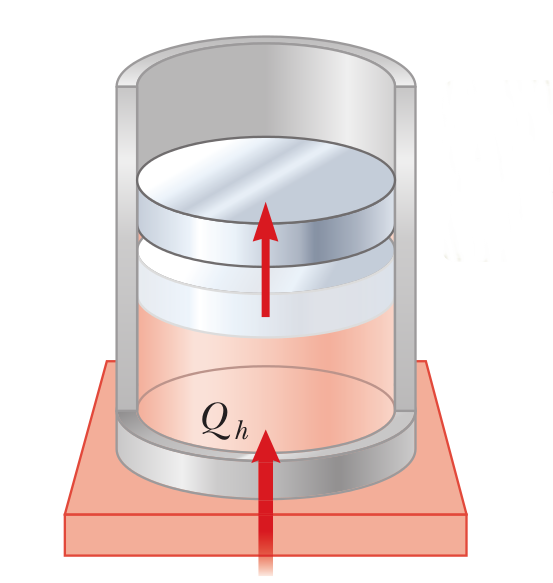
\includegraphics[height=0.45\textheight-32pt]{images/carnot-a.png}

            \(A \rightarrow B\) Expansão Isotérmica (\(T=\text{constante} \rightarrow Q_h = -W_1\))
        \end{column}

        \pause 
        \begin{column}{0.45\textwidth}
            \centering
            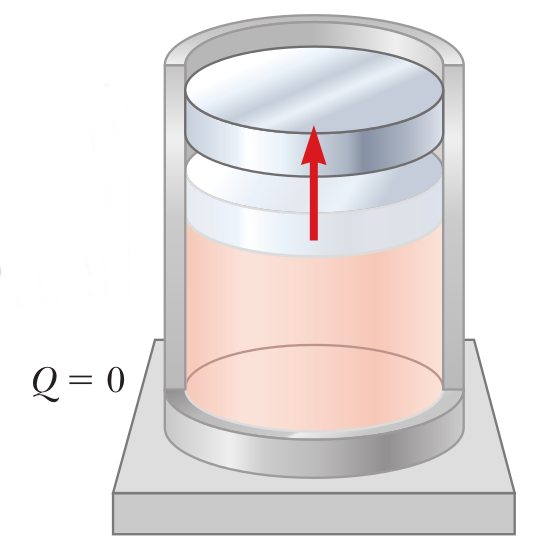
\includegraphics[height=0.45\textheight-32pt]{images/carnot-b.png}

            \(B \rightarrow C\) Expansão Adiabática (\(Q=0 \rightarrow \Delta E = W_2 \rightarrow T \downarrow \))
        \end{column}
    \end{columns}

    \begin{columns}
        \pause 
        \begin{column}{0.45\textwidth}
            \centering
            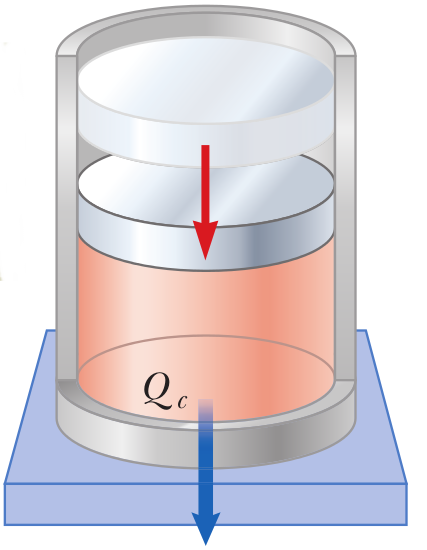
\includegraphics[height=0.45\textheight-32pt]{images/carnot-c.png}

            \(C \rightarrow D\) Compressão Isotérmica (\(T=\text{constante} \rightarrow Q_c = -W_3\))
        \end{column}

        \pause 
        \begin{column}{0.45\textwidth}
            \centering
            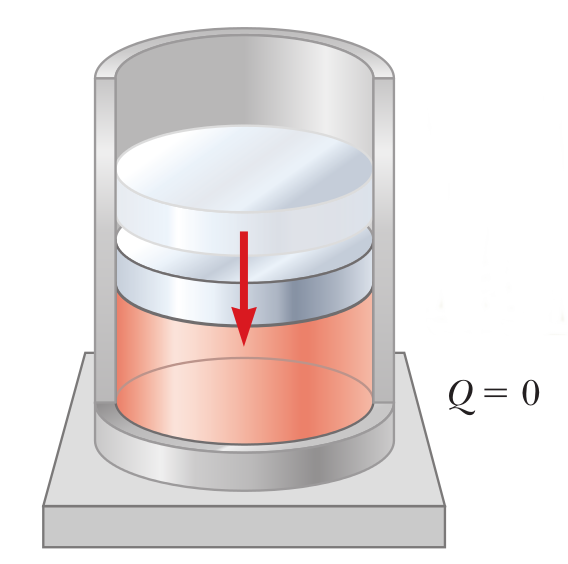
\includegraphics[height=0.45\textheight-32pt]{images/carnot-d.png}

            \(D \rightarrow A\) Compressão Adiabática (\(Q=0 \rightarrow \Delta E = W_4 \rightarrow T \uparrow \))
        \end{column}
    \end{columns}
\end{frame}

\begin{frame}
    \frametitle{Diagrama \(PV\) do ciclo de Carnot}
    \centering
    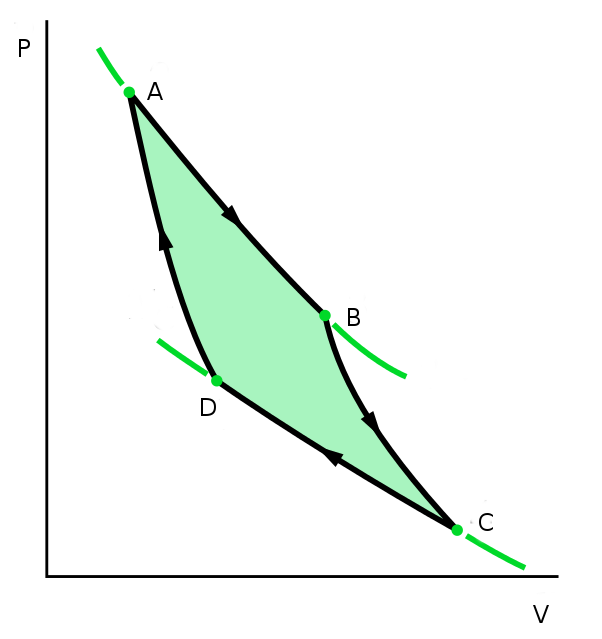
\includegraphics[height=\textheight-27pt]{images/carnot-ciclo.png}
\end{frame}

\begin{frame}{Exercícios do \textbf{Tipler}, capítulo 18}
    \centering
    \includegraphics<+>[width=\textwidth]{images/Captura de tela de 2024-03-05 11-38-10.png}
\end{frame}

% \begin{frame}{Segunda lei da termodinâmica}
%     \begin{block}{Enunciado de Kelvin}
%         Nenhum sistema pode absorver calor de um único reservatório e
%         convertê-lo inteiramente em trabalho sem que resultem outras variações
%         no sistema e no ambiente que o cerca
%     \end{block}

%     \pause
%     \begin{block}{Enunciado de Clausius}
%         Um processo cujo único resultado efetivo seja o de retirar calor de um
%         reservatório frio e liberar a mesma quantidade de calor para um
%         reservatório quente é impossível
%     \end{block}
% \end{frame}

% \begin{frame}{Atividade}
%     \begin{itemize}
%         \item Vale 15\% da N3
%         \item Grupo de no máximo 2 alunos
%         \item Pode ser digitado ou manuscrito
%         \item Fazer uma pesquisa sobre:
%             \begin{itemize}
%                 \item Teorema de Carnot
%                 \item Ciclo de Carnot
%                 \item Eficiência do ciclo de Carnot
%             \end{itemize}
%         \item  Entrega até o dia 21/03/2024
%     \end{itemize}
% \end{frame}

% \begin{frame}{Atividade}
%     \begin{itemize}
%         \item Vale 15\% da N3
%         \item Grupo de no máximo 2 alunos
%         \item Pode ser digitado ou manuscrito
%         \item Fazer uma pesquisa sobre:
%             \begin{itemize}
%                 \item Enunciado de Clausius
%                 \item Enunciado de Kelvin-Planck
%                 \item Equivalência entre os enunciados
%             \end{itemize}
%         \item  Entrega até o dia 21/03/2024
%     \end{itemize}
% \end{frame}

% \begin{frame}{Lista de exercícios para a prova 3}
%     \begin{itemize}
%         \item Problemas 43, 44, 45 e 46 do capítulo 18 do Halliday
%         \item Problemas 77, 79, 80, 81 e 82  do capítulo 18 do \textbf{Tipler}
%         \item A prova terá entre 4 problemas da lista com \textit{valores
%             numéricos modificados}
%         \item A prova será individual mas poderá haver \textit{consulta} entre alunos
%     \end{itemize}
% \end{frame}

% \begin{frame}{Exercícios do \textbf{Tipler}, capítulo 18}
%     \centering
%     \includegraphics<+>[width=\textwidth]{images/Captura de tela de 2024-03-20 09-32-41.png}

%     \includegraphics<+>[width=\textwidth]{images/Captura de tela de 2024-03-20 09-32-52.png}

%     \includegraphics<+>[width=\textwidth]{images/Captura de tela de 2024-03-20 09-33-11.png}

%     \includegraphics<+>[width=\textwidth]{images/Captura de tela de 2024-03-20 09-33-25.png}

%     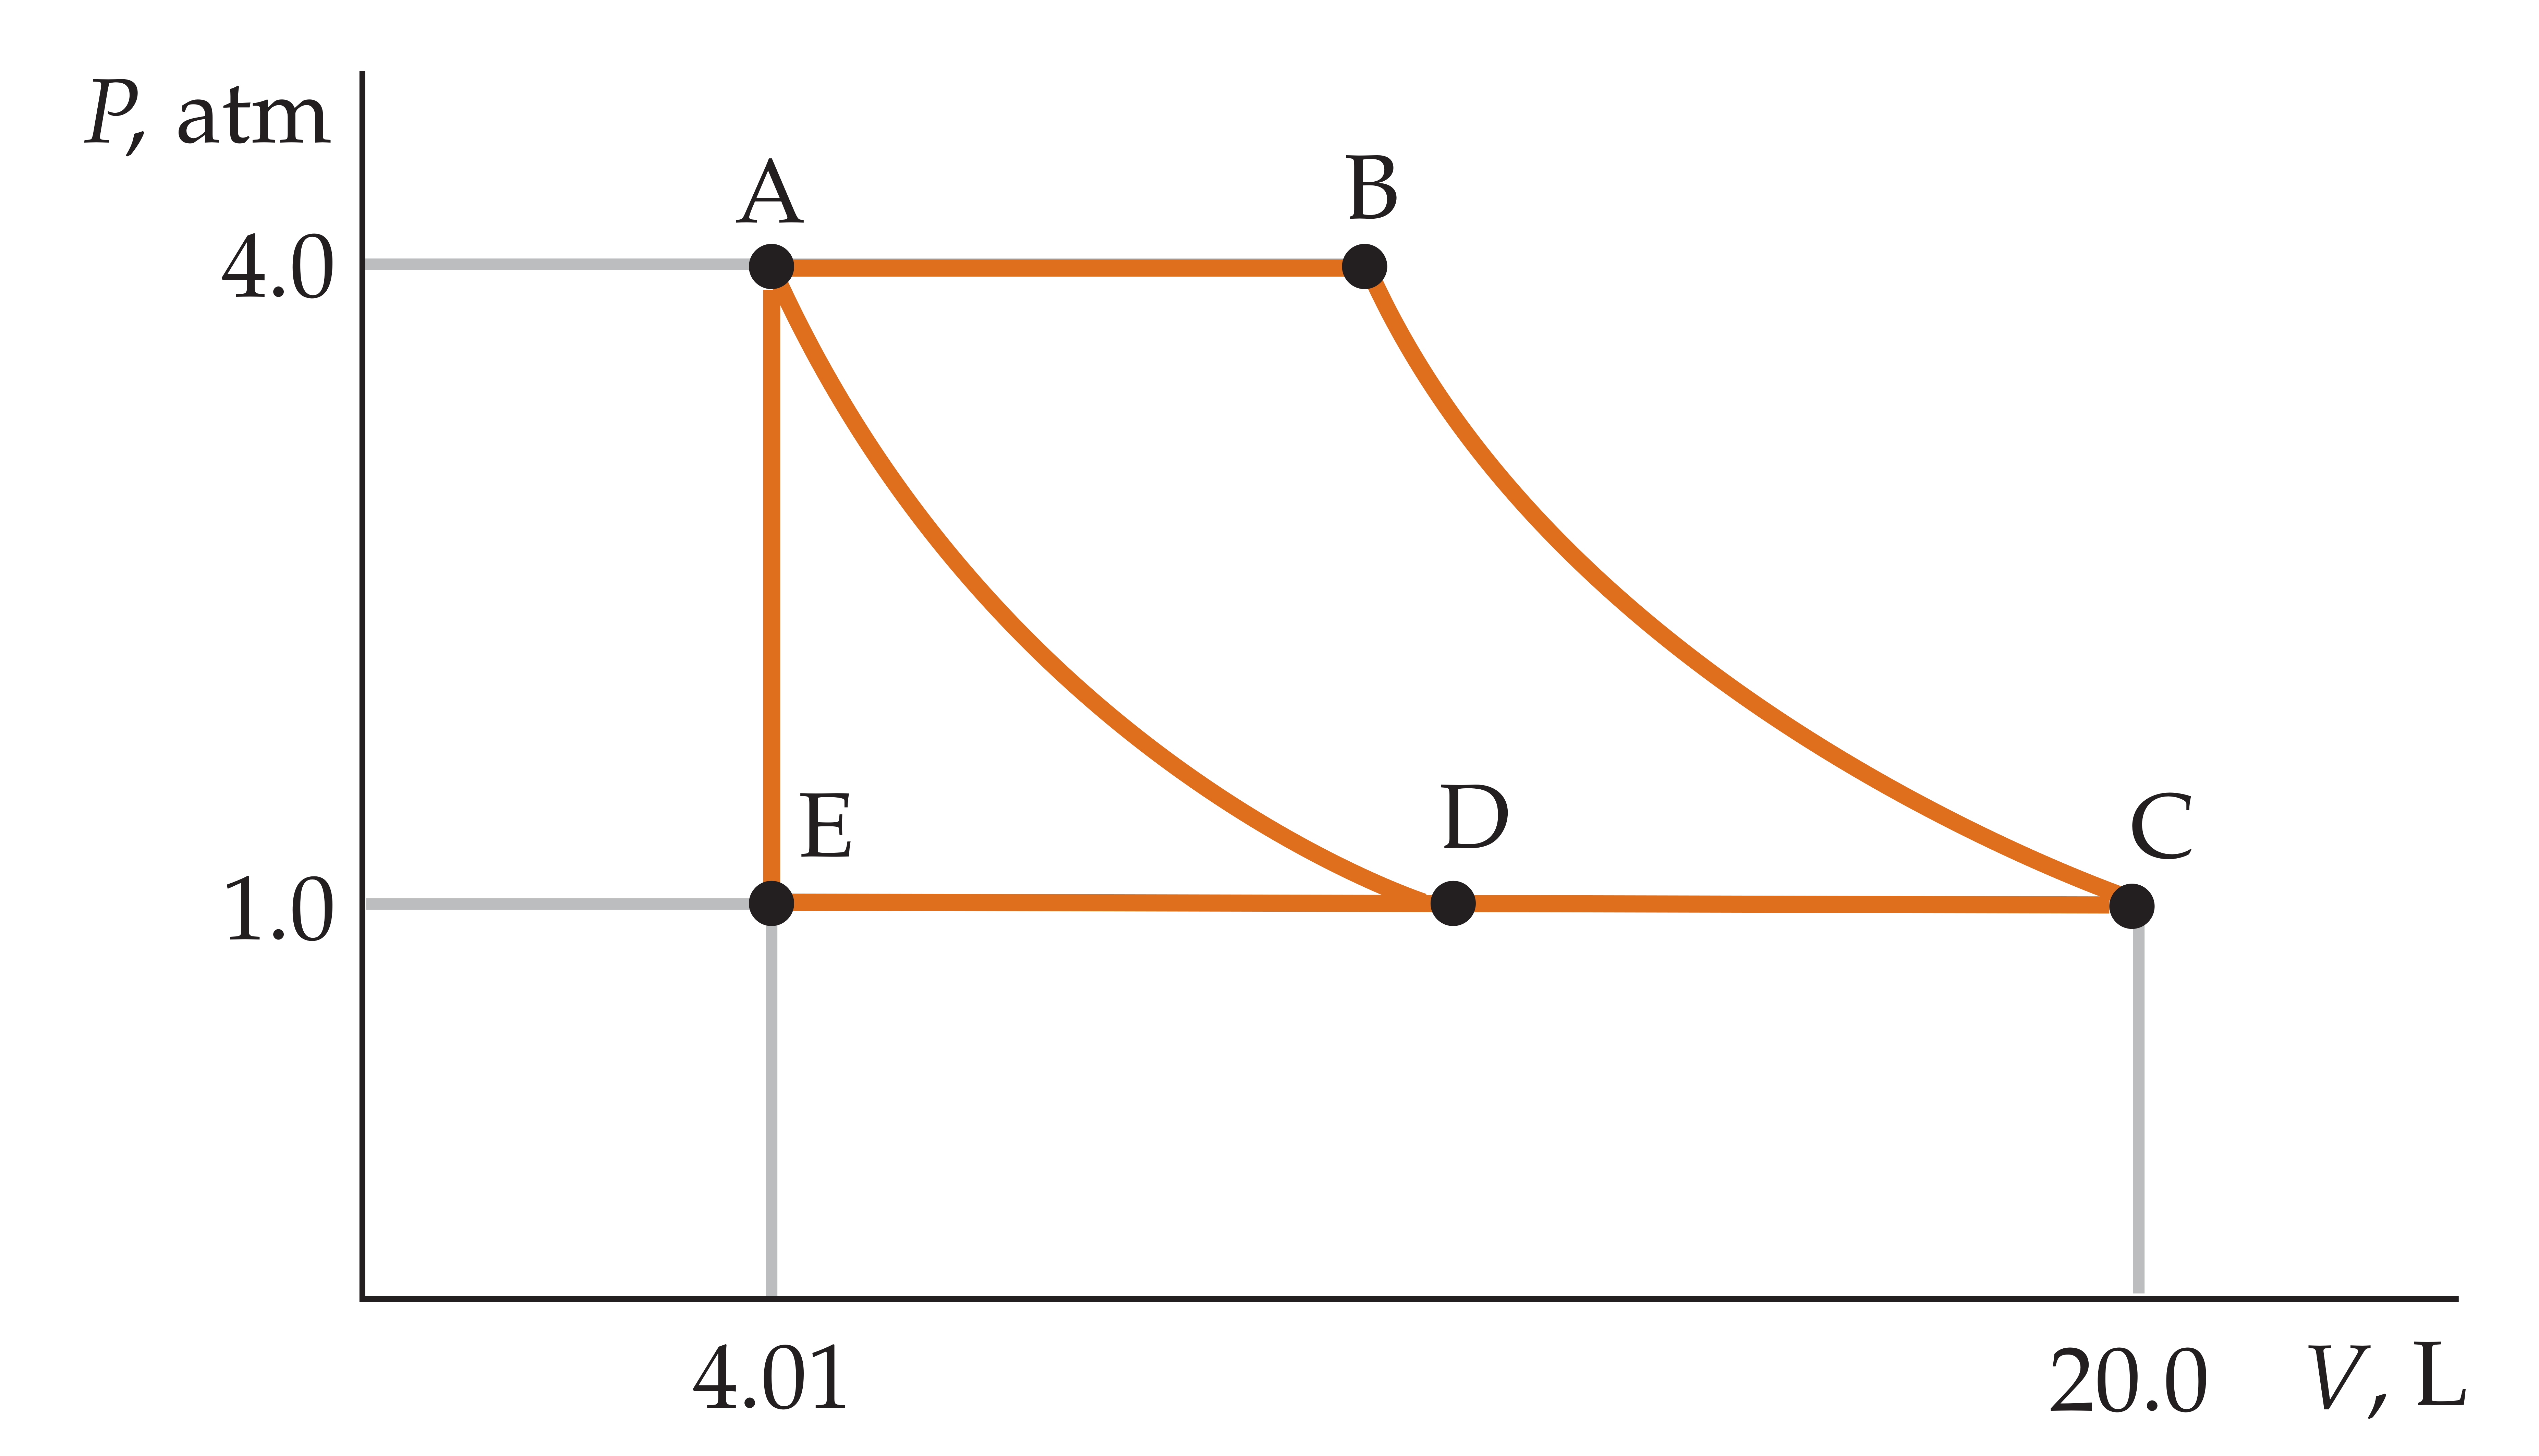
\includegraphics[width=\textwidth-133pt*\real{1.74}]{images/figura_18-25.png}

%     \textbf{FIGURA 18-25 Problemas 79, 80, 81 e 82}
% \end{frame}

\end{document}
